% TODO list - chapter #2 - updated 12/08/2020

% 0.) Add Pagnanin corrections
% 2.) add Michelson interf. and Young double pinhole references to the coherence chapter.

\begin{refsection}

%-------------------------------------------------------------------------
%-------------------------------------------------------------------------
\chapter{On a new kind of rays}\label{sec:x-rays}
%-------------------------------------------------------------------------
%-------------------------------------------------------------------------
%X-rays are electromagnetic radiation situated between the energies \todo{(X)}~$\mathrm{keV}$ and \todo{(XXX)}~$\mathrm{keV}$, or, equivalently, wavelengths of 2~\r{A} to 0.1~\r{A}

Hard X-rays are electromagnetic radiation with wavelength below\footnote{The choice of wavelength or enrgy to limit soft-, tender- and hard- X-rays is rather arbitrary. The conversion of energy to wavelength in practical unities is isually one by as $\text{E}(\text{keV})=12.38/\lambda(\text{\r{A}})$} 2~\r{A}. From their discovery in 1895 by W. C. R\"{o}ntgen [\cite{Roentgen1896}], the first observation of synchrotron radiation (SR) in 1947 [\cite{Elder1947}], the first (late 1950's and early 1960's), second (late 1970's and early 1980's), third (end of 1980's and early 1990's) and the fourth generation (late 2000's and early 2010's) of accelerator-based X-ray sources, a large amount of efforts was put into increasing the brilliance and consequently, the coherent fraction of the produced radiation [\cite{Robinson2015}]. This chapter is dived into three main parts. The first part introduces the concept of brilliance and connects it to the coherent fraction of synchrotron radiation emission, presenting undulators as the mains source of coherent X-rays in a synchrotron radiation facilities. In the second part of this chapter, the scalar wave theory is presented as a framework for modelling X-ray propagation through free-space and optical elements. Some definitions regarding optical coherence are also presented. The last part of this chapter deals with simulation strategies based on the degree of spatial coherence of the radiation.
%-------------------------------------------------------------------------
%-------------------------------------------------------------------------
\section{From the Hittorf's tube to the EBS}\label{sec:sources_intro}
%-------------------------------------------------------------------------
%-------------------------------------------------------------------------
Since the discovery\footnote{Professor W. C. R\"{o}ntgen has published his first notes on the discovery of X-rays in January 1896 in [\cite{Roentgen1896}]. In March the same year, R\"{o}ntgen went on to publish some additional notes on his discovery [\cite{Roentgen1896a}]. Further observations of the X-ray properties were later published in [\cite{Roentgen1897}].} of X-rays in late November 1895 by W. C. R\"{o}ntgen [\cite{Roentgen1896}] up to the concept and implementation of the fourthgeneration high-energy synchrotron light sources in the second half of the 2010's [\cite{Eriksson2016}], there has been an Herculean amount of work directed to increasing a key energy-dependent quality parameter of x-ray sources, called brilliance\footnote{Although a common jargon in X-ray science and technology, the term brilliance is not unanimously agreed upon. For an insightful discussion on the terminology, please refer to the discussion in [\cite{Mills2005}] and to the Chapter~3.9 and Table~3.1 in [\cite{Talman2006}]. Eq.~\ref{eq:brilliance} is an approximation result. For an accurate calculation of the brilliance, please, refer to [\cite{Walker2019}].}:
\begin{equation}\label{eq:brilliance}
   \mathcal{B}_0 = \frac{\varphi}{4\pi^2\epsilon_\mathrm{h}\epsilon_\mathrm{v}},
\end{equation}{}
where $\varphi$ is the X-ray photon flux for a given bandwidth $\Delta\mathrm{E}/\mathrm{E}=0.001$ centred at energy E,  given in $(\mathrm{ph}/\mathrm{s}/0.1\%\mathrm{bw.})$. Both $\epsilon_\mathrm{h}$ and $\epsilon_\mathrm{v}$ refer to the photon-beam emittances in the horizontal and vertical planes, respectively. The beam emittance is defined as:
\begin{equation}
    \epsilon_{\mathrm{h,v}}\equiv\Sigma_{\mathrm{h,v}}\cdot\Sigma_{\mathrm{h,v}}'.
\end{equation}{}
Here $\Sigma_{\mathrm{h,v}}$ stands for the beam size and $\Sigma'_{\mathrm{h,v}}$ is the photon-beam divergence. The usual unit used for the beam size is $(\mathrm{mm})$ and for beam divergence is $(\mathrm{mrad})$, hence brilliance is commonly given in $(\mathrm{ph}/\mathrm{s}/0.1\%\mathrm{bw.}/\mathrm{mm}^2/\mathrm{mrad}^2)$ [\cite{Kim1986}]. It is clear from Eq.~\ref{eq:brilliance} that increasing the brilliance means increasing the spectral photon flux $\varphi$ and/or reducing the photon-beam emittance in both horizontal and vertical directions ($\epsilon_\mathrm{h}$ and $\epsilon_\mathrm{v}$), i.e. having a smaller and more collimated X-ray source.
%-------------------------------------------------------------------------
%-------------------------------------------------------------------------
\subsection{X-ray sources}\label{sec:sources}
%-------------------------------------------------------------------------
%-------------------------------------------------------------------------
Two main processes are responsible for generating X-rays: acceleration of charged particles, in particular, electrons; and the change by an electron from a higher atomic or ionic energy level to a lower one.

In the very early X-ray sources such as the Hittorf's tube used by R\"{o}ntgen\footnote{On the opening sentence of his most important work \textit{"On a new kind of rays"}, R\"{o}ntgen mentions that X-rays can be produced by [sic.] \textit{"an electric discharge passing through a Hittorf's tube or a well-exhausted Lenard's or Crook's tube"} [\cite{Roentgen1896}].} or any modern X-ray tube (electron-impact X-ray sources) both processes generate X-rays: Bremsstrahlung by rapid deceleration of fast electrons, generating a broad-band smooth spectrum; and characteristic radiation (X-ray fluorescence), responsible for narrow spikes in the spectrum. Although modern sources can focus the electron-beam into the target (anode), reducing the source size considerably, the emission of X-rays happens in a large solid angle, $2\pi~(\mathrm{steradians})$. The emission angle, in conjunction with the fact that the X-ray flux is limited by the low current of electrons, makes X-ray tubes very-low brilliance sources  [\cite[\textit{§1.6} \& \textit{§2}]{Michette1993}].

\begin{figure}[t]
    \centering
    {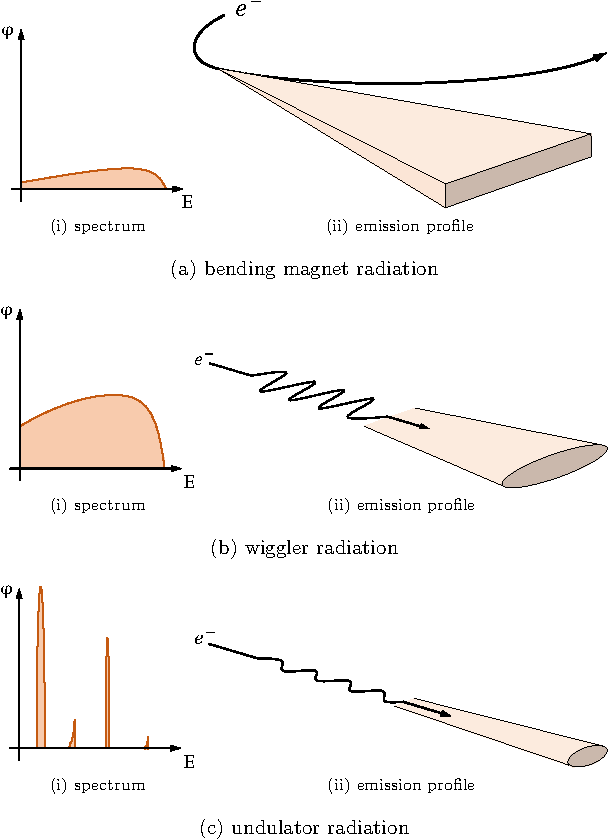
\includegraphics[width=.55\linewidth]{figures/ch02/x-ray_sources.pdf}}
    \caption[Synchrotron radiation emission]{Sketch of the three main sources of synchrotron radiation. On the left-handed side the photon-flux $\varphi$ as a function of energy $\mathrm{E}$ is shown. The right-hand side shows the electron ($e^-$) trajectory and the accompanying emission profile. Figure adapted from Figs.~5.1-5.3 in [\cite{Attwood1999}] and Fig.~1.2 from [\cite{Clarke2004}].}
    \label{fig:emission}
\end{figure}

In accelerator-based X-ray sources, more specifically, storage-ring-like facilities\footnote{Linear accelerators are also used as a source of intense synchrotron radiation, in particular in free-electron lasers (XFELs) [\cite{Huang2007}].}, (ultra-relativistic\footnote{At an energy of $\sim$11.43~MeV, the electron reaches $v/c = 99.9\%$ and at roughly 36.13~MeV the ratio is $v/c = 99.99\%$, where $v$ is the particle velocity and $c$ is the speed of light. Storage rings dedicated to synchrotron radiation operate at least above a few hundred MeV.}) electrons are usually chosen for generating X-rays as their low rest mass means that they emit by far the most radiation for a given particle energy. Charged particles in storage rings are subjected to a magnetic field perpendicular to the direction of motion and this causes the particle to move in a circular trajectory (centripetal acceleration). If the particle is non-relativistically accelerated, the emitted radiation is described by the Larmor pattern (torus-shaped profile), which shows no radiation in the direction of acceleration. However, for a particle in the ultra-relativistic regime, the Lorentz-transformed radiation pattern shows that the (synchrotron) radiation pattern is very peaked in the forward direction with a narrow angular divergence (cf. Fig.~\ref{fig:emission}) [\cite{Jackson1998}].

There are three main families of X-ray sources in a synchrotron facility: bending magnets (BM's), necessary structures in the storage ring to deflect the electron-beam transversely to its motion direction and keep it in a closed trajectory by applying a constant magnetic field or gradient. They produce a smooth broad-band spectrum and the photon-beam footprint is very large as both the source and divergence\footnote{The typical emission angle of synchrotron radiation is given by $1/\gamma$, where $\gamma$ is the Lorentz factor. For an electron in a storage ring: $\gamma=1957\cdot\mathrm{E(GeV)}$, with $\mathrm{E(GeV)}$ being the electron energy [\cite[\textit{§2.2.1}]{Als-Nielsen2011}].} sizes are very large. Historically, BMs have been used as the primary source of X-rays in first- and second-generation light-sources\footnote{The first generation of synchrotron light sources is usually attributed to the parasitic use of high-energy physics accelerators. The second-generation marks the beginning of fully-dedicated machines for synchrotron radiation.}. The bending magnet radiation spectrum and profile are shown in Fig.~\ref{fig:emission}(a)~and~(b). Storage rings are a multi-edge polygon where at each vertex sits a bending magnet gently deflecting the electron-beam keeping the electrons in a closed loop. The distance between two adjacent dipole magnets is called a straight section and is where insertion devices are placed.

Insertion devices (IDs) are periodic magnetic structures that sinusoidally deflect the electron-beam transversely to its direction of motion. IDs can be sub-grouped into two categories based on the amplitude of the electron motion inside them and their magnetic period: wigglers have a higher magnetic field applied to the electron-beam causing the amplitude of electron motion to be large. The magnetic period in a wiggler is considered to be large. This generates a broad-band spectrum several times more intense than that of a bending magnet (higher flux). The beam footprint is also very large: the source size is big and the beam has a higher divergence than that of the natural divergence of synchrotron radiation from BMs. Figures~\ref{fig:emission}(c)~and~(d) show the spectrum and emission profile of a wiggler insertion device. The last member of the family of X-ray sources in particle-accelerators is the undulator. In it, the amplitude of the electron motion is much smaller than inside a wiggler. This is because in the undulators a less intense magnetic field is applied to the electrons and due to the fact that the magnetic period is usually smaller than the one of a wiggler. The small excursion of the electrons inside the undulator accounts for a small photon source size with low divergence. Due to the low electron-motion amplitude, constructive interference between the emitted radiation occurs and the spectrum of an undulator is composed of narrow-band peaks called undulator harmonics\footnote{If the observer is on-axis with the electron motion, only odd harmonics are observed. Away from the emission axis, even harmonics start being observed [\cite[\textit{§4.2}]{Clarke2004}].}. Figures~\ref{fig:emission}(d)~and~(e) show the spectrum and emission profile of an undulator. The advent of storage rings specially designed to accommodate ID's marks the third generation of synchrotron light sources, from which the ESRF - European Synchrotron Research Facility (1994) in France is the pioneering machine, followed by the APS - Advanced Photon Source (1996) in the USA and the SPring-8 - Super Photon ring-8~GeV (1999) in Japan. 

%-------------------------------------------------------------------------
%-------------------------------------------------------------------------
\subsection{High brilliance X-ray sources}\label{sec:brilliance}
%-------------------------------------------------------------------------
%-------------------------------------------------------------------------

The small photon source size and low divergence of the X-rays emitted by an undulator make it a great candidate for generating high-brilliance X-ray beams. As Eq.~\ref{eq:brilliance} suggests, increasing the brilliance can be done by two different strategies: increasing the photon flux, which is done by increasing the electron current in the storage ring; and/or by reducing the photon-beam emittance.

The radiation profile (beam sizes and divergences) emitted by an undulator is given by the convolution between electron-beam profile and the radiation pattern specific of the X-ray source\footnote{This is true for any accelerator-based X-ray source - cf. chapter "3.10 - Photon beam features inherited from the electron beam" in [\cite{Talman2006}].}: 
\begin{subequations}\label{eq:undulator}
    \begin{align}   
    \Sigma_{\mathrm{h,v}} &= \sigma_{e_{\mathrm{h,v}}}*\sigma_{u_{\mathrm{h,v}}},\\
    \Sigma'_{\mathrm{h,v}} &= \sigma'_{e_{\mathrm{h,v}}}*\sigma'_{u_{\mathrm{h,v}}}.
    \end{align}
\end{subequations}{}
Here $\Sigma_{\mathrm{h,v}}$ and $\Sigma'_{\mathrm{h,v}}$ are the already defined photon-beam size and divergence. The $\sigma_{e_{\mathrm{h,v}}}$ and $\sigma'_{e_{\mathrm{h,v}}}$ represent the electron-beam size and divergence. Lastly, $\sigma_{u_{\mathrm{h,v}}}$ and $\sigma'_{u_{\mathrm{h,v}}}$ are the specific radiation pattern size and divergence of the insertion device - these are the obtained by calculating the emission of a filament electron-beam (negligible dimension and divergence) passing through the magnetic field of the insertion device. Once designed, the specific radiation pattern of an undulator\footnote{The specific radiation pattern of an undulator is a function of its magnetic period, number of periods, magnetic field, storage ring energy and X-ray emission-wavelength.} is considered to be a fundamental property of the insertion device\footnote{In the literature, there is a great variety of formulae for calculating the specific radiation pattern size and divergence [\cite{Kim1986, Kim1989, Tanaka2009, Elleaume2013}]. Different assumptions, approximations and fits are done on their derivation. It is important to state that those are approximations and should not be regarded as fundamental results - please, refer to the discussion in [\cite{Walker2019}]. The exact calculation of the radiation pattern can be done by computing the electric field of an electron subjected to an arbitrary magnetic field - cf. [\cite{Chubar1995, Chubar2001}] or by calculating the Wigner-function for synchrotron radiation [\cite{Bazarov2012}] as in [\cite{Tanaka2014}].}.

A closer look into Eqs.~\ref{eq:undulator} allows one to suppose three distinct regimes for the photon-beam characteristics: a) $\epsilon_{e_{\mathrm{h,v}}}\gg\epsilon_{u_{\mathrm{h,v}}}$ in this regime, the photon-beam characteristics are dominated by the electron-beam, which is well approximated by a Gaussian distribution. This is usually the case for horizontal emittance in third-generation synchrotrons; b) an intermediate state where the electron-beam emittance $\epsilon_{e_{\mathrm{h,v}}}$ is comparable to $\epsilon_{u_{\mathrm{h,v}}}$ leading to a photon-beam profile with clear contributions of both the electron-beam and specific radiation pattern of the undulator; c) the electron-beam emittance can be further reduced so that $\epsilon_{e_{\mathrm{h,v}}}\ll\epsilon_{u_{\mathrm{h,v}}}$ and the photon-beam profile is dominated by the undulator's specific radiation pattern. Since $\epsilon_{u_{\mathrm{h,v}}}$ is a fundamental limit, efforts to reducing the electron-beam beyond that limit will not have any impact in the photon-beam profile. Mathematically, the three emittance regimes can be expressed as:
\begin{subequations}\label{eq:emittances}
    \begin{align}
           \epsilon_{\mathrm{h,v}}&\Big\vert_{\epsilon_{e_{\mathrm{h,v}}}\gg\epsilon_{u_{\mathrm{h,v}}}}  \simeq\Big(\sigma_{e_{\mathrm{h,v}}}*\delta_{u_{\mathrm{h,v}}}\Big)\Big(\sigma'_{e_{\mathrm{h,v}}}*\delta_{u_{\mathrm{h,v}}}\Big)=\sigma_{e_{\mathrm{h,v}}}\sigma'_{e_{\mathrm{h,v}}},\\
           \epsilon_{\mathrm{h,v}}&\Big\vert_{\epsilon_{e_{\mathrm{h,v}}}\sim\epsilon_{u_{\mathrm{h,v}}}}
           \simeq\Big(\sigma_{e_{\mathrm{h,v}}}*\sigma_{u_{\mathrm{h,v}}}\Big)\Big(\sigma'_{e_{\mathrm{h,v}}}*\sigma'_{u_{\mathrm{h,v}}}\Big)=\Sigma_{\mathrm{h,v}}\Sigma'_{\mathrm{h,v}},\\
           \epsilon_{\mathrm{h,v}}&\Big\vert_{\epsilon_{e_{\mathrm{h,v}}}\ll\epsilon_{u_{\mathrm{h,v}}}}
           \simeq \Big(\delta_{e_{\mathrm{h,v}}}*\sigma_{u_{\mathrm{h,v}}}\Big)\Big(\delta_{e_{\mathrm{h,v}}}*\sigma'_{u_{\mathrm{h,v}}}\Big)=\sigma_{u_{\mathrm{h,v}}}\sigma'_{u_{\mathrm{h,v}}}.
    \end{align}
\end{subequations}{}
Where $\delta$ represents the Dirac function. The electron-beam emittance matching to the undulator's specific radiation pattern is shown in Fig.~\ref{fig:matching}. Fourth-generation synchrotron light-sources\footnote{The fourthgeneration synchrotron light sources or ultra-low emittance machines have been proposed as early as the 1990's [\cite{Einfeld1996, Einfeld2014}], but were deemed to be technologically unfeasible for high-energy storage rings [\cite{Ropert2000, Elleaume2003}]. Overcoming the technological barriers [\cite{Borland2014}] was essential in paving the way for high energy storage rings with ultra-low emittance [\cite{Bei2010, Eriksson2016}]. The first machines to come online using the multi-bend-achromat design (MBA) are the MAX-IV in Sweden (2016) and the SIRIUS in Brazil (2019) - the former operating with two storage rings: $1.5~\mathrm{GeV}$ and $3~\mathrm{GeV}$ and the latter operating at $3~\mathrm{GeV}$. The ESRF upgrade programme has opted for a hybrid-multi-bend-achromat (HMBA) magnetic lattice for its new storage ring [\cite{Biasci2014}] and it is the first of its kind to operate at high-energies ($6~\mathrm{GeV}$). The lattice concept behind the Extremely Brilliant Source (ESRF-EBS) has it's origins in 2006 with the SuperB project for an electron-positron collider [\cite{Raimondi2017}] and in early 2020 has produced the first X-rays.} use emittance-matching as the main source of increasing the X-ray brightness\footnote{This is due to the fact that with the new storage-ring designs (multi-bend-achromat and its variations), the electron-beam emittance can be routinely reduced one to two orders of magnitude, when compared to current third-generation light sources. To obtain equivalent gain in brightness by just increasing the electron-beam current is very challenging in function of collective effects (coherent and incoherent). On the top of that, there are thermal load issues on the vacuum system and on the beamline optics, that is, the X-ray transport system to the sample. This footnote is the result of discussions with Pedro F. Tavares (MAX-IV, Sweden)  and Boaz Nash (RadiaSoft LLC, USA).} [\cite[\textit{§21.8.1}]{Wiedemann2015}].

\begin{figure}[t]
    \centering
    {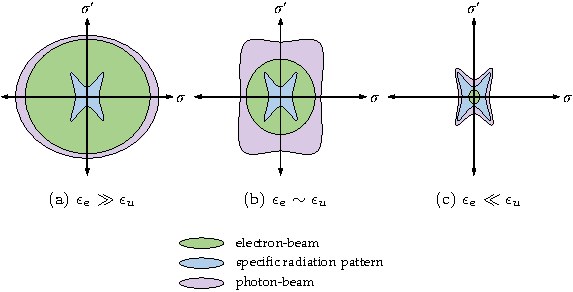
\includegraphics[width=.6\linewidth]{figures/ch02/emittance.pdf}}
    \caption[Emittance matching]{Matching of the electron-beam emittance to the undulator specific radiation pattern to increase the photon-beam brightness, where $\sigma$ stands for beam size and $\sigma'$ for beam divergence. Adapted from Fig.~21.20 in [\cite{Wiedemann2015}].}
    \label{fig:matching}
\end{figure}

%-------------------------------------------------------------------------
%-------------------------------------------------------------------------
\subsection{Undulators as a primary source of coherent X-rays}\label{sec:undulators}
%-------------------------------------------------------------------------
%-------------------------------------------------------------------------

 Let's consider the case of a filament electron-beam passing through a planar undulator. The associated emission is symmetric and $\sigma_{u_{\mathrm{h}}}=\sigma_{u_{\mathrm{v}}}=\sigma_{u}$ and $\sigma'_{u_{\mathrm{h}}}=\sigma'_{u_{\mathrm{v}}}=\sigma'_{u}$. Because the electron bunch has negligible emittance $\epsilon_e$ in both horizontal and vertical directions, the photon-beam emittance is given by $\epsilon_\mathrm{h,v}=\sigma_{u}\sigma'_u=\epsilon_\mathrm{u}$. The associated brilliance of such a filament beam is given by:
\begin{equation}\label{eq:brilliance_coherent}
\mathcal{B}_0 = \frac{\varphi}{4\pi^2\epsilon^2_{u}}
\end{equation}{}
Since the emission of a filament electron-beam is fully-coherent, it makes sense to define a coherent photon flux of a zero-electron-emittance-beam. From Eq.~\ref{eq:brilliance_coherent}:
\begin{equation}\label{eq:coherent_flux}
\varphi_\mathrm{coh.} = 4\pi^2\epsilon^2_{u}\mathcal{B}_0=\Bigg(\frac{\lambda}{2}\Bigg)^2\mathcal{B}_0.
\end{equation}{}
It is important to mention that the right-hand side of Eq.~\ref{eq:coherent_flux} is valid for any symmetric electric field distribution at any value of undulator detuning and it does not depend on a Gaussian approximation of the undulator specific radiation pattern [\cite{Walker2019}]. Although Eq.~\ref{eq:coherent_flux} implies that $\epsilon_u = \sigma_u\sigma'_u =\lambda/4\pi$, it has been demonstrated that diffraction-limited photon-emittance approaches asymptotically $\lambda/2\pi$ instead [\cite{Khubbutdinov2019}]. One can define the coherent fraction as the ratio between the coherent flux $\varphi_\mathrm{coh.}$ (Eq.~\ref{eq:coherent_flux}) and the nominal photon-flux $\varphi = 4\pi^2\epsilon_\mathrm{h}\epsilon_\mathrm{v}\mathcal{B}_0$ (Eq.~\ref{eq:brilliance}):
\begin{equation}\label{eq:coherent_fraction}
\zeta =  \frac{\varphi_\mathrm{coh.}}{\varphi}=\frac{\epsilon^2_{u}}{\epsilon_\mathrm{h}\epsilon_\mathrm{v}}.
\end{equation}{}
Eq.~\ref{eq:coherent_fraction} allows to deduce that by reducing the electron-beam emittance, the coherence fraction is increased (cf. Eqs.~\ref{eq:emittances}). An important conclusion to be drawn is that emittance-matching as a form of increasing the photon-beam brilliance in fourth-generation synchrotrons increases the X-ray beam transverse (spatial) coherence\footnote{Please, refer to §\ref{sec:optical_coherence}~-~\textit{\nameref{sec:optical_coherence}} for a definition of spatial and temporal coherence.\label{note:coherence}}.

%-------------------------------------------------------------------------
%-------------------------------------------------------------------------
\subsubsection*{Temporal Coherence}
%-------------------------------------------------------------------------
%-------------------------------------------------------------------------

Lastly, the temporal coherence\footnote{See footnote \ref{note:coherence}.} of the synchrotron radiation should be addressed. Without further conditioning, the radiation emitted on the X-ray region exhibits low temporal coherence for high energies. Spectral filtering with monochromators increases the temporal coherence at the expense of photon-flux reduction. Compressing the electron bunch length also offers an increased temporal coherence for X-rays, as coherent synchrotron radiation (CSR) naturally appears when the electron-beam bunch length is comparable to the radiation wavelength - cf. [\cite{Chubar2006}], [\cite[\textit{§3.8} \& \textit{§13}]{Talman2006}] and [\cite[\textit{§21.7}]{Wiedemann2015}]. 

%-------------------------------------------------------------------------
%-------------------------------------------------------------------------
\subsection*{Recommended literature}
%-------------------------------------------------------------------------
%-------------------------------------------------------------------------

The correct description of the electron-beam inside each different source of X-rays in a storage ring is of primary importance for accurate modelling of the radiation spectrum and photon spatial distribution, with consequences to X-ray optical design.
An extensive review on particle accelerator physics is given by [\cite{Duke2000}] and by [\cite{Wiedemann2015}]. An in-depth look into X-rays from accelerator sources can be found in [\cite{Clarke2004}], in [\cite{Talman2006}] and in [\cite{Elleaume2013}].

The accurate calculation of the brightness from undulators in low-emittance accelerators and the coherence properties of the X-rays from them emitted is a vivid topic and a deeper look into it is offered by [\cite{Bazarov2012, Tanaka2014, Geloni2015, Geloni2008, Walker2019, Khubbutdinov2019}]. See also [\cite{Singer2014}].

\section{Physical optics}\label{sec:physical_optics}
\begin{figure}[t]
    \centering
    {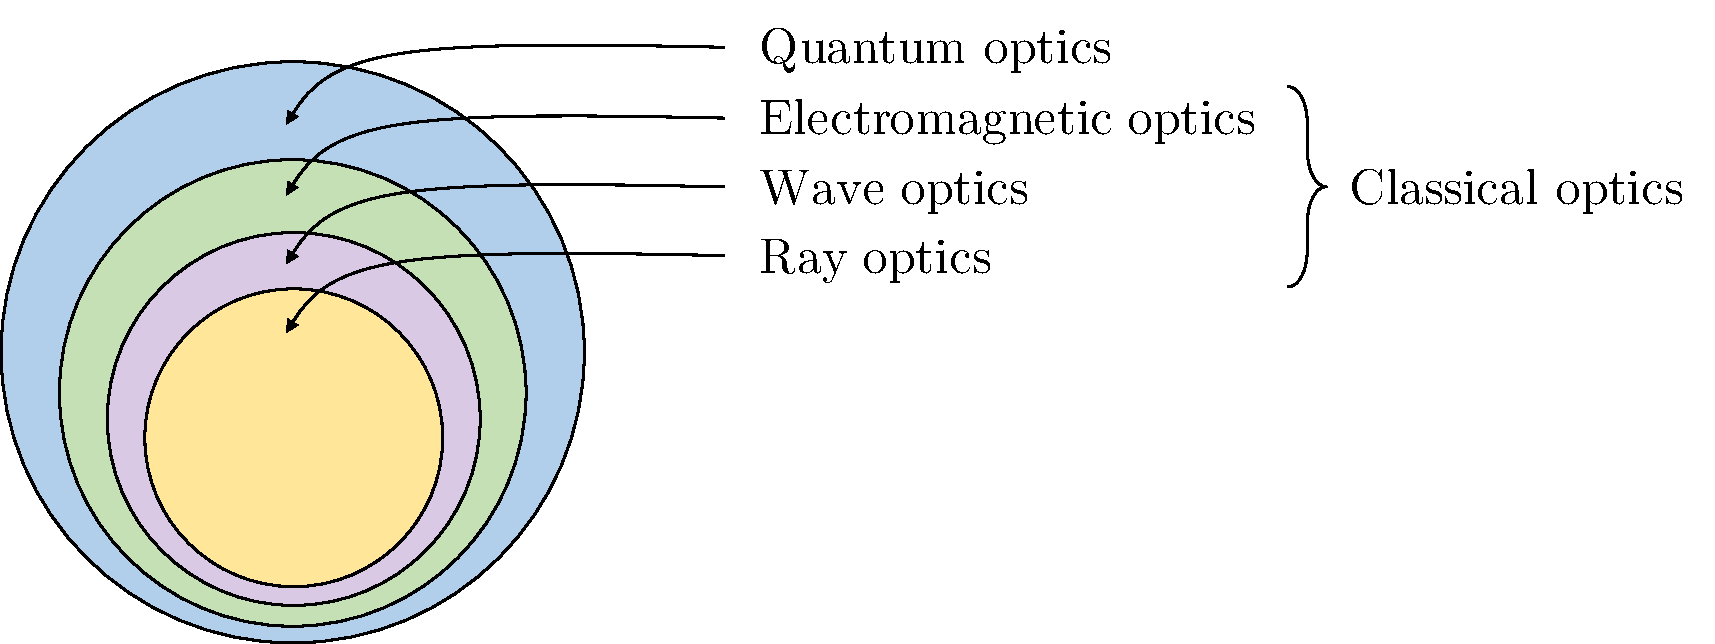
\includegraphics[width=.55\linewidth]{figures/ch02/optics.pdf}}
    \caption[Hierarchical optical theories]{Hierarchical optical theories. Optical modelling in the X-ray regime can be accurately represented in the realms of wave optics for most cases where coherence effects are present. Adapted from Fig.~1.0-1 in [\cite{Saleh2019}].}
    \label{fig:optical_theories}
\end{figure}
The increasing coherent fraction of X-rays from fourth-generation storage rings requires
an appropriate framework for their representation. Light can be described by an electromagnetic wave phenomenon governed by the Maxwell equations - cf. [\cite[\textit{§1.1}]{born_wolf1999}]:
\begin{subequations}\label{eq:Maxwell}
    \begin{align}
        \nabla\cdot\textbf{E} &= \frac{\rho}{\varepsilon}
                                       &&(\small{\text{Gau{\ss}'s~law}}),\\
        \nabla\cdot\textbf{B} &= 0 
                                       &&(\small{\text{Gau{\ss}'s law for magnetism}}),\\
        \nabla\times\textbf{E} &= -\frac{\partial}{\partial t}\textbf{B}
                                        &&(\small{\text{Faraday's law}}),\\
        \nabla\times\textbf{B} &= \mu\Bigg(\textbf{J}+\varepsilon\frac{\partial}{\partial t}\textbf{E}\Bigg)
                                       &&(\small{\text{Ampère's law modified by Maxwell}}).
    \end{align}
\end{subequations}{}
Where $\textbf{E}\equiv\textbf{E}(x,y,z,t)$ is the electric field, $\textbf{B}\equiv\textbf{B}(x,y,z,t)$ is the magnetic induction, $\varepsilon\equiv\varepsilon(x,y,z,t)$ and $\mu\equiv\mu(x,y,z,t)$ are the electric permittivity and magnetic permeability, $\rho\equiv\rho(x,y,z,t)$ is the charge density and $\textbf{J}\equiv\textbf{J}(x,y,z,t)$ is the current density. The operator $\nabla\cdot\bullet$ denotes the divergence of a vectorial field (scalar function) and $\nabla\times\bullet$ is the curl operator (vectorial function), where $\bullet$ is a generic vectorial field. The Cartesian coordinates $(x,y,z)$ and time $t$ have been omitted in favour of a more compact notation. Although electromagnetic optics provides the most complete framework for classical optical phenomena, it is possible to move away from the vectorial treatment of light towards a scalar wave theory in order treat a large variety of relevant optical phenomena. This simplified treatment of light is commonly referred to scalar wave optics or physical optics (cf. Fig.~\ref{fig:optical_theories} for the hierarchical representaion of optical theories). X-ray wave-fields in free-space are discussed in §\ref{sec:free-space}~-~\textit{\nameref{sec:free-space}} and their transmission through generic refractive optical elements is discussed in §\ref{sec:thin_element}~-~\textit{\nameref{sec:thin_element}}.

%-------------------------------------------------------------------------
%-------------------------------------------------------------------------
\subsection{Free-space propagation}\label{sec:free-space}
%-------------------------------------------------------------------------
%-------------------------------------------------------------------------

In order to describe wave-fields in free-space under the scalar theory, one usually starts\footnote{The developments in §\ref{sec:free-space}~-~\textit{\nameref{sec:free-space}} are inspired by the derivations from [\cite[\textit{§1}]{Paganin2006}] and [\cite[\textit{§3} \& \textit{§4}]{Goodman2017}].} by obtaining the Maxwell equations for free-space (vacuum). This is done considering that the medium where the wave-fields exist are uncharged and non-conducting, which is done by letting $\rho=0$ and $\textbf{J}=\textbf{0}$ in Eqs.~\ref{eq:Maxwell}a and~\ref{eq:Maxwell}d:
\begin{subequations}\label{eq:Maxwell_free}
    \begin{align}
        \nabla\cdot\textbf{E} &= \textbf{0},\\
        \nabla\times\textbf{B} &= \mu_0\varepsilon_0\frac{\partial}{\partial t}\textbf{E}.
    \end{align}
\end{subequations}{}
Where $\varepsilon_0$ and $\mu_0$ are the vacuum electric permittivity and magnetic permeability. Direct consequences of deriving the scalar theory for waves in vacuum is that the medium is assumed being linear (permittivity is linear), isotropic (permittivity is independent of polarisation direction), homogeneous (permittivity is constant within the region of propagation), nondispersive (permittivity is independent of wavelength throughout the region of interest) and, finally, nonmagnetic (the magnetic permeability constant and equal to $\mu_0$) [\cite[\textit{§3.2}]{Goodman2017}]. 

%-------------------------------------------------------------------------
%-------------------------------------------------------------------------
\subsubsection*{The wave-equation}
%-------------------------------------------------------------------------
%-------------------------------------------------------------------------

The d'Alembert wave-equation for the electric field can be obtained by applying the curl operator $\nabla\times\bullet$ to both sides of Faraday's law, using the vector calculus identity $\nabla\times(\nabla\times\bullet)=\nabla(\nabla\cdot\bullet)-\nabla^2\bullet$ to the electric field $\textbf{E}$, and making use of the Maxwell equations for free-space (Eqs.~\ref{eq:Maxwell} and~\ref{eq:Maxwell_free}):
\begin{equation}\label{eq:Evectorial_waveeq}
    \Bigg(\varepsilon_0\mu_0\frac{\partial^2}{\partial t^2} - \nabla^2\Bigg)\textbf{E}=\textbf{0}.
\end{equation}
 The same reasoning can be applied to the magnetic induction $\textbf{B}$:
\begin{equation}\label{eq:Bvectorial_waveeq}
    \Bigg(\varepsilon_0\mu_0\frac{\partial^2}{\partial t^2} - \nabla^2\Bigg)\textbf{B}=\textbf{0}.
\end{equation}
Each vectorial component of $\textbf{E}$ and $\textbf{B}$ satisfies individually a scalar form of the wave-equation and each of the individual components are uncoupled from each other - cf. [\cite[\textit{§1.1}]{Paganin2006}]. It is possible to define a (complex) scalar field $u(x,y,z,t)$ representing any of the components of $\textbf{E}$ or $\textbf{B}$ such that:
\begin{equation}\label{eq:Scalar_WE}
    \Bigg(\frac{1}{c^2}\frac{\partial^2}{\partial t^2} - \nabla^2\Bigg)u=0.
\end{equation}
with $c=1/\sqrt{\varepsilon_0\mu_0}$ (speed of light in vacuum). This complex scalar solution of the d'Alembert equation can be spectrally decomposed as a superposition of monochromatic fields using the Fourier transform:
\begin{equation}\label{eq:spectral_decomposition}
    u(x,y,z,t)=\frac{1}{\sqrt{2\pi}}\int\limits_{-\infty}^\infty{U(x,y,z)\exp{(-i\omega t)}~\mathrm{d}\omega}
\end{equation}
The argument of the integral in Eq.~\ref{eq:spectral_decomposition} implies that the monochromatic field can be written down as a product of a spatial dependent function and a time dependent function (separation of variables) [\cite[\textit{§1.2}]{Paganin2006}]. Plugging Eq.~\ref{eq:spectral_decomposition} in Eq.~\ref{eq:Scalar_WE}:
\begin{equation}\label{eq:Helmholtz}
    (\nabla^2 + k^2)U(x,y,z) = 0,
\end{equation}
where $k=\omega/c=2\pi/\lambda$ is the wavevenumber and $\lambda$, the associated wavelength. Eq.~\ref{eq:Helmholtz} is know as the Helmholtz equation. Given a volume in space and boundary conditions, the scalar diffraction theory consists in finding the solutions to q.~\ref{eq:Helmholtz} [\cite[\textit{§1.2}]{Paganin2006}]. One of the simplest solutions to the Helmholtz equation in free-space is the so-called plane-wave:
\begin{equation}\label{eq:planewave}
    U(\textbf{r}) = A\exp(-i\textbf{k}\cdot\textbf{r})=A\exp[-i(k_xx+k_yy+k_zz)],
\end{equation}
where $A$ is a complex constant (complex envelope), $\textbf{k}=(k_x, k_y, k_z)$ is the wavevector such as $\vert\textbf{k}\vert=k$ and $\textbf{r}=(x,y,z)$. A second solution is spherical wave:
\begin{equation}\label{eq:spherical}
    U(\textbf{r}) = \frac{A}{r}\exp(-ikr),
\end{equation}
here $\vert\textbf{r}\vert=r$ is the distance from the origin of the wavefront. Two other common waves are often found in modelling of optical systems. Defining henceforth the $z-$axis as the optical axis, the paraboloidal wave is given by:
\begin{equation}\label{eq:parabolic}
    U(\textbf{r}) = \frac{A}{z}\exp(-ikz)\exp{\Bigg[-ik\frac{x^2 + y^2}{2z}\Bigg]},
\end{equation}
Eq.~\ref{eq:parabolic} is a paraxial\footnote{Consider a spherical wave with $\textbf{r}=(x,y,z)$ and that $\vert\textbf{r}\vert=r=\sqrt{x^2 + y^2 +z^2}$ and take a sufficiently large coordinate along the $z-$axis (optical axis). The paraxial approximation of the spherical wave can be obtained by choosing points in the $xy-$plane near enough the $z-$axis so that $\sqrt{x^2+y^2}\ll z$ holds. It follows that $r=z\sqrt{1+(x^2+y^2)/z^2}$ can be expanded in a Taylor series: $r\approx z+(x^2+y^2)/2z$ and directly plugged into the exponent in Eq.~\ref{eq:spherical} leading to Eq.~\ref{eq:parabolic} [\cite[\textit{§2.2}]{Saleh2019}]. The paraxial approximation of the spherical wave is also called the Fresnel approximation.\label{note:fresnel}} approximation of the spherical wave defined by Eq.~\ref{eq:spherical}; and the Gaussian beam\footnote{Take the paraboloidal wave as defined by Eq.~\ref{eq:parabolic}. Evaluating it along the optical axis at a position $z^+=z+\Delta z$ also yields a solution to the paraxial Helmholtz equation (cf. Eq.~\ref{eq:Helmholtz_paraxial}) even if $\Delta z$ is a purely imaginary number [\cite[\textit{Exercise 2.2-2}]{Saleh2019}]. The Gaussian beam can be obtained from the paraboloidal wave by substituting $z$ in Eq.~\ref{eq:parabolic} by $z-iz_0$, for a real $z_0$ [\cite[\textit{§3.1}]{Saleh2019}].}:
\begin{equation}\label{eq:gaussian}
    U(\textbf{r})=-i\frac{A}{z_0}\frac{w_0}{W(z)}\exp{\Bigg[-\frac{x^2+y^2}{W^2(z)}\Bigg]}\exp\Bigg[ -ikz - ik\frac{x^2 +y^2}{2R(z)}+i\varphi(z)\Bigg],
\end{equation}
where $z_0$ is the so-called Rayleigh range and:
\begin{subequations}\label{eq:gaussian_parameters}
    \begin{align}
        W(z) &= w_0\sqrt{1+\Bigg(\frac{z}{z_0}\Bigg)^2}&&(\small{\text{beam~width}}),\\
        R(z) &= z \Bigg[1+ \Bigg(\frac{z}{z_0}\Bigg)^2\Bigg] &&(\small{\text{wavefront-radius-of-curvature}}),\\
        \varphi(z) &= \tan^{-1}\Bigg(\frac{z}{z_0}\Bigg) &&(\small{\text{Gouy~phase}}),\\
        w_0 &= \sqrt{\frac{\lambda z_0}{\pi}} &&(\small{\text{beam~width~at~the~waist}}).
    \end{align}
\end{subequations}{}
Both the paraboloidal wave and Gaussian beam do not, however, formally satisfy the Helmholtz equation as defined by Eq.~\ref{eq:Helmholtz}. They do obey a paraxial form of the Helmholtz wave-equation. This assumes a plane wave as defined in Eq.~\ref{eq:planewave} can be modulated by a complex envelope $A(\textbf{r})$ that slowly varies along a distance $\lambda=2\pi/k$ along the optical axis $z$. It can be shown\footnote{The complete derivation of the paraxial wave-equation can be found in [\cite[\textit{§2.2.C}]{Saleh2019}].} that plugging this modulated plane-wave in the Helmholtz equation (Eq.~\ref{eq:Helmholtz}) leads to:
\begin{equation}\label{eq:Helmholtz_paraxial}
    \Bigg(i2k\frac{\partial}{\partial z}-\nabla^2_T\Bigg)A=0.
\end{equation}
where $\nabla^2_T\equiv\partial^2/\partial x^2 + \partial^2/\partial y^2$ is the transverse Laplace operator. Eq.~\ref{eq:Helmholtz_paraxial} is the paraxial Helmholtz equation [\cite[\textit{§2.2}]{Saleh2019}]. Determining the evolution in space of the solutions to the Helmholtz equation (Eq.~\ref{eq:Helmholtz}) or the paraxial Helmholtz equation (Eq.~\ref{eq:Helmholtz_paraxial}) is the core of what is called scalar diffraction theory.


\begin{figure}[t]
    \centering
    {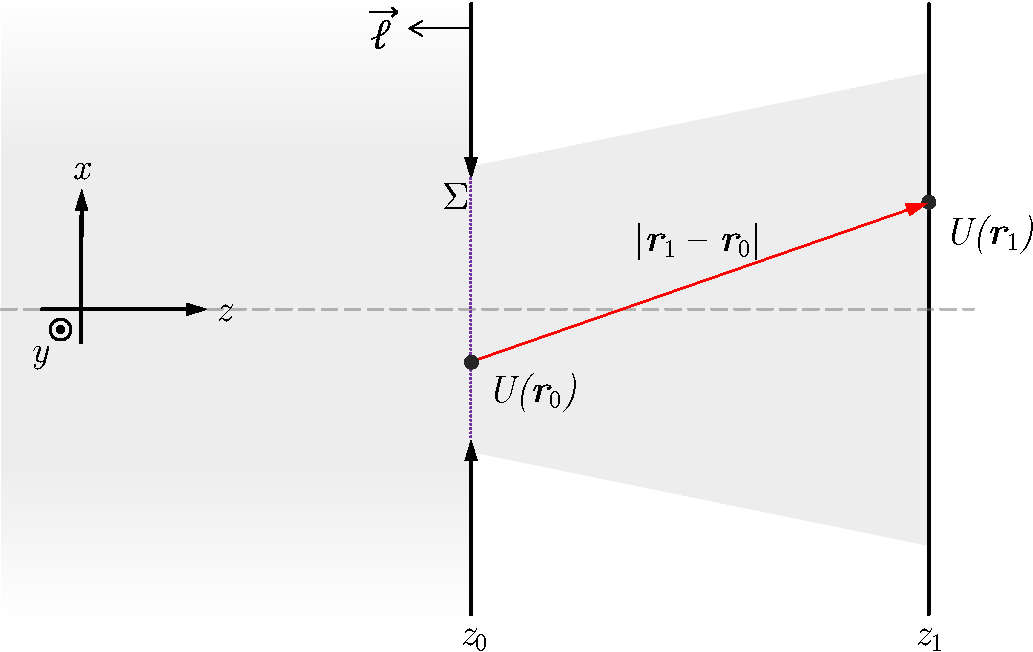
\includegraphics[width=.45\linewidth]{figures/ch02/diffraction_geometry.pdf}}
    \caption[Scalar diffraction problem geometry]{Scalar diffraction problem geometry. $\Sigma$ represents the input plane, where the electric field is completely defined, that is, $U(x_0, y_0, z_0)$ is known for all $(x_0, y_0, z_0)$, $\ell$ is a orthonormal vector to $\Sigma$. Scalar diffraction theory concerns the calculation of an electric field $U(x_1, y_1, z_1)$ in the output plane with the knowledge of it in the input plane.}
    \label{fig:diffraction}
\end{figure}

\newpage
%-------------------------------------------------------------------------
%-------------------------------------------------------------------------
\subsubsection*{Fresnel diffraction}
%-------------------------------------------------------------------------
%-------------------------------------------------------------------------

Consider a Cartesian coordinate system where the $z-$axis is the optical axis (cf. Fig~\ref{fig:diffraction}), suppose a transverse component of a wave-field complying with Eq.~\ref{eq:Helmholtz} can be completely described at a position $z_0$, that is, $U(x,y,z_0)$ is known for all the $xy-$plane. The wave-field distribution in a parallel plane at a position $z_1$ of the optical axis can be calculated using the first Rayleigh-Sommerfeld diffraction equation [\cite[\textit{Eq.~3-42}]{Goodman2017}]:
\begin{equation}\label{eq:Huygens-Fresnel}
    U(\textbf{r}_1) = \frac{k}{i2\pi}\iint\limits_{\Sigma}{U(\textbf{r}_0)\frac{\exp{(ik\vert\textbf{r}_1 - \textbf{r}_0\vert)}}{\vert\textbf{r}_1 - \textbf{r}_0\vert}\cos{(\vec{\ell},\textbf{r}_1 - \textbf{r}_0)}~\mathrm{d}s},
\end{equation}
where $\textbf{r}_0=(x_0,y_0,z_0)$, $\textbf{r}_1=(x_1,y_1,z_1)$, $\vec{\ell}$ is a normal vector parallel to the optical axis and $\Sigma$ is the $xy-$plane in $z_0$ where the integration takes place - cf. Fig~\ref{fig:diffraction}. Eq.~\ref{eq:Huygens-Fresnel} assumes that $\vert\textbf{r}_1 - \textbf{r}_0\vert\gg\lambda$ and is often referred to as the Huygens-Fresnel principle\footnote{Eq.~\ref{eq:Huygens-Fresnel} expresses the wave-field evaluated in $\textbf{r}_1$, that is, $U(\textbf{r}_1)$ as a sum of spherical wave-fronts originating from a secondary sources modulated by $U(x_0,y_0,z_0)$ at each point $\textbf{r}_0$ within the aperture $\Sigma$.} [\cite[\textit{§3.7}]{Goodman2017}]. In the paraxial approximation $\cos{(\vec{\ell},\textbf{r}_1 - \textbf{r}_0)}\approx1$ and $\vert\textbf{r}_1 - \textbf{r}_0\vert=\sqrt{(x_1-x_0)^2+(y_1-y_0)^2+L^2}\approx L +[(x_1-x_0)^2+(y_1-y_0)^2]/2L$, where $L=z_1-z_0$ with $L\gg\vert x_1-x_0\vert$ and $L\gg\vert y_1-y_0\vert$. The latter is know as the Fresnel approximation. Eq.~\ref{eq:Huygens-Fresnel} can be simplified to:
\begin{equation}\label{eq:Fresnel}
    U(x_1,y_1,z_1)=\frac{k\exp{(ikL)}}{2\pi i L}\iint\limits_{-\infty}^{\hspace{8pt}\infty}{U(x_0,y_0,z_0)\exp{\Bigg\{\frac{ik}{2L}\big[(x_1-x_0)^2+(y_1-y_0)^2 \big]\Bigg\}}~\mathrm{d}x_0\mathrm{d}y_0},
\end{equation}
which is know as the Fresnel diffraction integral [\cite[\textit{§4.2}]{Goodman2017}]. The accuracy of Eq.~\ref{eq:Fresnel} is limited by the Taylor expansion of $\vert\textbf{r}_1 - \textbf{r}_0\vert=L\sqrt{1+\rho^2/L^2}$, where  $\rho = \sqrt{(x_1-x_0)^2+(y_1-y_0)^2}$, which is usually usually truncated on the linear term\footnote{The Taylor series expansion at $v=0$ is $\sqrt{1+v}=1+\frac{v}{2}-\frac{v^2}{8}+\frac{v^3}{16}+\mathcal{O}(v^4)$ and it converges for $\vert v\vert<1$.}, provided that the phase induced by the quadratic term of the expansion is much less than the Rayleigh's quarter-wave criterion, which limits the maximum phase error to $\pi/4$ radians [\cite[\textit{§9.3}]{born_wolf1999}]. Neglecting high-order terms in the approximation of the square-root in Eq.~\ref{eq:Fresnel} can be done if:
\begin{equation}\label{eq:accuracy_Fresnel}
    \sqrt[3]{\frac{\rho^4}{\lambda}}\ll z.
\end{equation}

%-------------------------------------------------------------------------
%-------------------------------------------------------------------------
\subsubsection*{Fraunhofer diffraction}
%-------------------------------------------------------------------------
%-------------------------------------------------------------------------

Still analysing Eq.~\ref{eq:Fresnel}, the quadratic term in the exponential part of the integrand can be expanded and rearranged: 
\begin{multline}\label{eq:Fresnel_2}
    U(x_1,y_1,z_1)=\frac{k\exp{(ikL)}}{2\pi i L}\exp{\Bigg[ \frac{ik}{2L}(x_1^2+y_1^2)\Bigg]}\cdot\\
    \cdot\iint\limits_{-\infty}^{\hspace{8pt}\infty}{U(x_0,y_0,z_0)\exp{\Bigg[\frac{ik}{2L}\big(x_0^2+y_0^2-2x_1x_0-2y_1y_0)\Bigg]}~\mathrm{d}x_0\mathrm{d}y_0}.
\end{multline}
Applying the Rayleigh's quarter-wave criterion to the $k(x_0^2+y_0^2)/2L$ term in Eq.~\ref{eq:Fresnel_2}:
\begin{equation}\label{eq:accuracy_Fraunhofer}
    4\frac{x_0^2 +y_0^2}{\lambda}\ll z,
\end{equation}
which allows to further simplify Eq.~\ref{eq:Fresnel} into:
\begin{multline}\label{eq:Fraunhofer}
    U(x_1,y_1,z_1)=\frac{k\exp{(ikL)}}{2\pi i L}\exp{\Bigg[ \frac{ik}{2L}(x_1^2+y_1^2)\Bigg]}\cdot\\
    \cdot\iint\limits_{-\infty}^{\hspace{8pt}\infty}{U(x_0,y_0,z_0)\exp{\Bigg[-\frac{ik}{L}\big(x_1x_0+y_1y_0)\Bigg]}~\mathrm{d}x_0\mathrm{d}y_0},
\end{multline}
Eq.~\ref{eq:Fraunhofer} is know as the Fraunhofer diffraction integral.

%-------------------------------------------------------------------------
%-------------------------------------------------------------------------
\subsubsection*{Numerical computation of the Fresnel and Fraunhofer diffraction}
%-------------------------------------------------------------------------
%-------------------------------------------------------------------------

The numerical calculation of the diffraction integrals is a vast subject and has been addressed by a plurality of authors [\cite{DArcio:94}], [\cite{Kelly2014}], [\cite[\textit{§5}]{Goodman2017}], [\cite{Buitrago-Duque:19}] and [\cite{Chubar2019}], among many others. This arises from the fact that unless the resulting field $U(x_1,y_1,z_1)$ has an analytical representation, numerically calculating the integrals in Eq.~\ref{eq:Fresnel} and Eq.~\ref{eq:Fraunhofer} will forcefully result in tackling issues like replicas and aliasing. This comes from the fact that the diffraction integrals are intimately connected with the Fourier analysis. 

Upon closer inspection, it is apparent that the Fresnel diffraction integral (Eq.~\ref{eq:Fresnel}) is a two-dimensional convolution type integral [\cite[\textit{§2.1}]{Goodman2017}]:
\begin{equation}\label{eq:conv}
    g(x,y) * h(x,y) = \iint\limits_{-\infty}^{\hspace{8pt}\infty}{g(u,v)h(x-u,y-u)~\mathrm{d}u\mathrm{d}v},
\end{equation}{}
which can be computed by invoking the convolution theorem:
\begin{equation}\label{eq:conv_theorem}
    g(x,y) * h(x,y) = \mathcal{F}^{-1}\big\{\mathcal{F}\{g(x,y)\}\cdot\mathcal{F}\{h(x,y)\}\big\},
\end{equation}{}
where $\mathcal{F}\{\bullet\}$ is the two-dimensional Fourier transform and $\mathcal{F}^{-1}\{\bullet\}$ denotes inverse Fourier transform:
\begin{subequations}\label{eq:Fourier}
    \begin{align}
        \mathcal{F}\{g\} &= \iint\limits_{-\infty}^{\hspace{8pt}\infty}{g(x,y)\exp{\big[-i2\pi(f_xx+f_yy)\big]}~\mathrm{d}x\mathrm{d}y}\\
        \mathcal{F}^{-1}\{G\} &=\iint\limits_{-\infty}^{\hspace{8pt}\infty}{G(f_x,f_y)\exp{\big[i2\pi(f_xx+f_yy)\big]}~\mathrm{d}f_x\mathrm{d}f_y}.
    \end{align}
\end{subequations}{}
It is common to represent the Fourier analysis and syntheses as $\mathcal{F}\{g(x,y)\}\equiv G(f_x,f_y)$ and $\mathcal{F}^{-1}\{G(f_x,f_y)\}\equiv g(x,y)$, where $(f_x,f_y)$ are generally referred to as frequencies. For the Fresnel diffraction integral, the kernel of the convolution in Eq.~\ref{eq:conv_theorem}, that is $\mathcal{F}\{h(x,y)\}$, has analytical formulation:
% \begin{equation}\label{eq:kernel}
%     \mathcal{F}\{h(x_1,y_1)\} = \frac{k\exp{(ikL)}}{2\pi i L}\mathcal{F}\Bigg\{
%     \exp\bigg[\frac{ik}{2L}\big(x_1^2+y_1^2 \big)\bigg]\Bigg\} = \exp{(ikL)}\exp{\bigg[-\frac{i\pi^2 2L}{k} \big(f_x^2+f_y^2 \big)\bigg]},
% \end{equation}
\begin{equation}\label{eq:kernel}
     \frac{k}{2\pi i L}\mathcal{F}\{h(x,y)\} = \frac{k}{2\pi i L}\mathcal{F}\Bigg\{
    \exp\bigg[\frac{ik}{2L}\big(x^2+y^2 \big)\bigg]\Bigg\} = \exp{\bigg[-\frac{i2L\pi^2}{k} \big(f_x^2+f_y^2 \big)\bigg]},
\end{equation}
%with $f_x=x/(\lambda L)$ and $f_y=y/(\lambda L)$.
This formulation allows to calculate the Fresnel diffraction integral (Eq.~\ref{eq:Fresnel}) by means of the convolution theorem (Eq.~\ref{eq:conv_theorem}) by applying a Fourier transform to the input field, multiplying it by an analytical kernel and applying an inverse Fourier transform to the result. It is also evident that the Fraunhofer diffraction integral (Eq.~\ref{eq:Fraunhofer}) is a Fourier type integral, differing from Eq.~\ref{eq:Fourier}a by a multiplicative factor outside the integrand. 

\begin{figure}[t]
    \centering
    {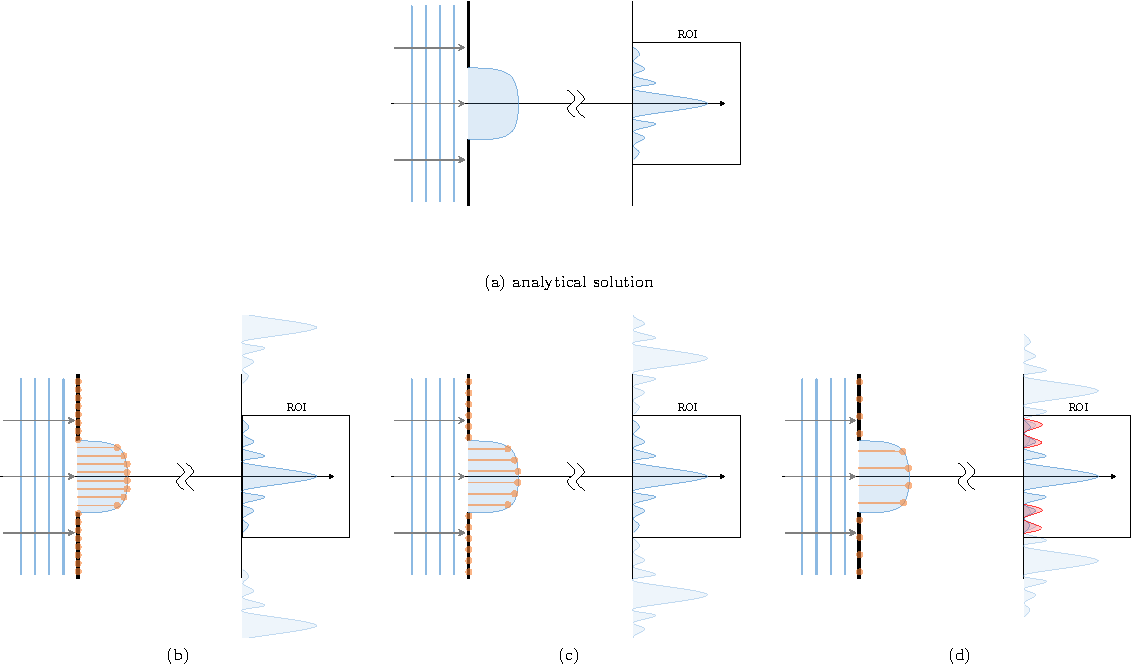
\includegraphics[width=1\linewidth]{figures/ch02/sampling_aliasing.pdf}}
    \caption[Replicas and aliasing]{Replicas and aliasing from numeric calculations of the diffraction integrals. (a) analytical solution of the integrals have no signal replicas. Sampling the input plane signal will introduce replicas in the output plane [\cite{Kelly2014}]. (b) appropriate sampling - cf. Eq.~5 in [\cite{Chubar2019}] - makes the unavoidable replicas further enough that cross-talk between them is negligible within the region of interest (ROI). (c) coarser sampling brings replicas closer up to a point that (d) replicas are so close that aliasing is eminent (red signal).}
    \label{fig:sampling}
\end{figure}

It should be clear, then, that the paraxial diffraction equations are intertwined with Fourier analysis. Numerically computation of the Fresnel or Fraunhofer diffraction implies \textit{a}-) sampling the input plane $U(x_0,y_0,z_0)$ and \textit{b}-) limiting its extent by either defining an aperture of finite extent or simply by cropping (truncating) the input field. It follows from sampling theory and the discrete Fourier transform (DFT) [\cite[\textit{§10}~\&~\textit{§11}]{Bracewell2000}] that sampling the input field causes replicas of the main signal to appear (cf. Fig.~\ref{fig:sampling}). Generally, the finer the sampling in the input plane, the further apart the replicas are. Consequently, the coarser the mesh gets, the closer they get up to a point that the replicas are close enough to each other that they start cross-talking. The interaction between the main signal and its replicas is called aliasing. Due to the finite extent of the input plane (either by limiting the signal with an aperture or by simply truncating it), it is inevitable that power from neighbouring replicas leak into each other. Sampling should be high enough as to make this inevitable cross-talk negligible [\cite{Kelly2014}]. On the other hand, a very large sampling leads to very inefficient calculations largely because of the size of the input and output planes - cf. considerations in [\cite[\textit{§5}]{Goodman2015}]. Efforts towards a memory and CPU efficient computation of the Fresnel free-space propagator in Fourier optics have been reported in [\cite{Chubar2019}].

%-------------------------------------------------------------------------
%-------------------------------------------------------------------------
\subsection{Transmission elements}\label{sec:thin_element}
%-------------------------------------------------------------------------
%-------------------------------------------------------------------------

The propagation of X-rays in the presence of matter can also be modelled with the Maxwell equations (Eqs.~\ref{eq:Maxwell}). It is possible to derive a Helmholtz equation in the presence of scatterers with a similar treatment given in the previous section, albeit considerably more algebraic - a detailed account of the derivation is given by [\cite[\textit{§2.1}]{Paganin2006}]. Restricting the analysis to linear isotropic non-magnetic materials where both the electric permittivity and magnetic permeability are independent of time (static medium) and considering again that the waves exist in a uncharged and non-conducting material,  that is, $\rho=0$ and $\textbf{J}=\textbf{0}$:
% \begin{subequations}\label{eq:dAllembert_inho_intermediate}
%     \begin{align}
%         \Bigg[\varepsilon(x,y,z)\mu_0\frac{\partial^2}{\partial t^2} - \nabla^2 \Bigg]\textbf{E}(x,y,z,t) &= -\nabla[\nabla\cdot\textbf{E}(x,y,z,t)], \\
%         \Bigg[\varepsilon(x,y,z)\mu_0\frac{\partial^2}{\partial t^2} - \nabla^2 \Bigg]\textbf{B}(x,y,z,t) &=
%         \frac{\nabla\varepsilon(x,y,z)}{\varepsilon(x,y,z)}\times[\nabla\times\textbf{B}(x,y,z,t)].
%     \end{align}
% \end{subequations}{}
% Eqs.~\ref{eq:dAllembert_inho_intermediate} can be reduced to\footnote{cf. Eqs.~2.18-2.21 in [\cite{Paganin2006}].}:
\begin{subequations}\label{eq:dAllembert_inho}
    \begin{align}
        \Bigg[\varepsilon(x,y,z)\mu_0\frac{\partial^2}{\partial t^2} - \nabla^2 \Bigg]\textbf{E}(x,y,z,t) &= \textbf{0}, \\
        \Bigg[\varepsilon(x,y,z)\mu_0\frac{\partial^2}{\partial t^2} - \nabla^2 \Bigg]\textbf{B}(x,y,z,t) &=\textbf{0}.
    \end{align}
\end{subequations}{}
considering that the scatterers are sufficiently slowly varying when compared to the radiation wavelength - cf. Eqs.~2.18-2.21 in [\cite{Paganin2006}]. Eqs.~\ref{eq:dAllembert_inho} resemble the vectorial wave-equations \ref{eq:Evectorial_waveeq} and \ref{eq:Bvectorial_waveeq}. This enables to give the same scalar treatment used for deriving the Helmholtz equation in free-space, that is, to propose a scalar field $u(x,y,z,t)$ such as:
\begin{equation}\label{eq:Scalar_WE_inho}
    \Bigg[\varepsilon(x,y,z)\mu_0\frac{\partial^2}{\partial t^2} - \nabla^2\Bigg]u=0,
\end{equation}
and spectrally decompose $u$ in its monochromatic Fourier components $U(x,y,z)\exp{(-i\omega t)}$ (cf. Eq.~\ref{eq:spectral_decomposition}):
\begin{equation*}
    u(x,y,z,t)=\frac{1}{\sqrt{2\pi}}\int\limits_{-\infty}^\infty{U(x,y,z)\exp{(-i\omega t)}~\mathrm{d}\omega}
\end{equation*}
This Fourier integral can be plugged into Eq.~\ref{eq:Scalar_WE_inho}, which leads to the Helmholtz equation in the presence of scatterers\footnote{cf. [\cite[\textit{Eq.~2.28}]{Paganin2006}].}:
\begin{equation}\label{eq:Helmholtz_inho}
    \big[\nabla^2 + k^2n^2(x,y,z)\big]U(x,y,z) = 0,
\end{equation}{}
where $n$ is the wavelength-dependent refractive index such that $n(x,y,z)^2\equiv\varepsilon(x,y,z)/\varepsilon_0$. This version of the Helmholtz equation for a inhomogeneous medium can rarely be solved exactly and approximations are necessary to handle Eq.~\ref{eq:Helmholtz_inho} [\cite[\textit{§2.1}]{Paganin2006}]. The same argument used to derive the paraxial Helmholtz equation (Eq.~\ref{eq:Helmholtz_paraxial}) can be applied here. Assuming a plane wave (Eq.~\ref{eq:planewave}) modulated by a complex envelope $A(\textbf{r})$ slowly varying along a distance $\lambda$ and plugging it into Eq.~\ref{eq:Helmholtz_inho}, one arrives to:
\begin{equation}\label{eq:Helmholtz_inho_paraxial}
    \Bigg\{2ik\frac{\partial}{\partial z}-\nabla^2_T+k^2\big[n^2(x,y,z)-1\big]\Bigg\}A=0.
\end{equation}{}
which is known as the paraxial Helmholtz equation in matter. Eq.~\ref{eq:Helmholtz_inho_paraxial} is compatible to the treatment used for propagating the wave-fields in free-space - cf. [\cite[\textit{Eq.~2.33}]{Paganin2006}]. Notice that Eq.~\ref{eq:Helmholtz_inho_paraxial} reduces to Eq.~\ref{eq:Helmholtz_paraxial} for $n=1$.

%-------------------------------------------------------------------------
%-------------------------------------------------------------------------
\subsubsection*{The projection approximation}
%-------------------------------------------------------------------------
%-------------------------------------------------------------------------

\begin{figure}[t]
    \centering
    {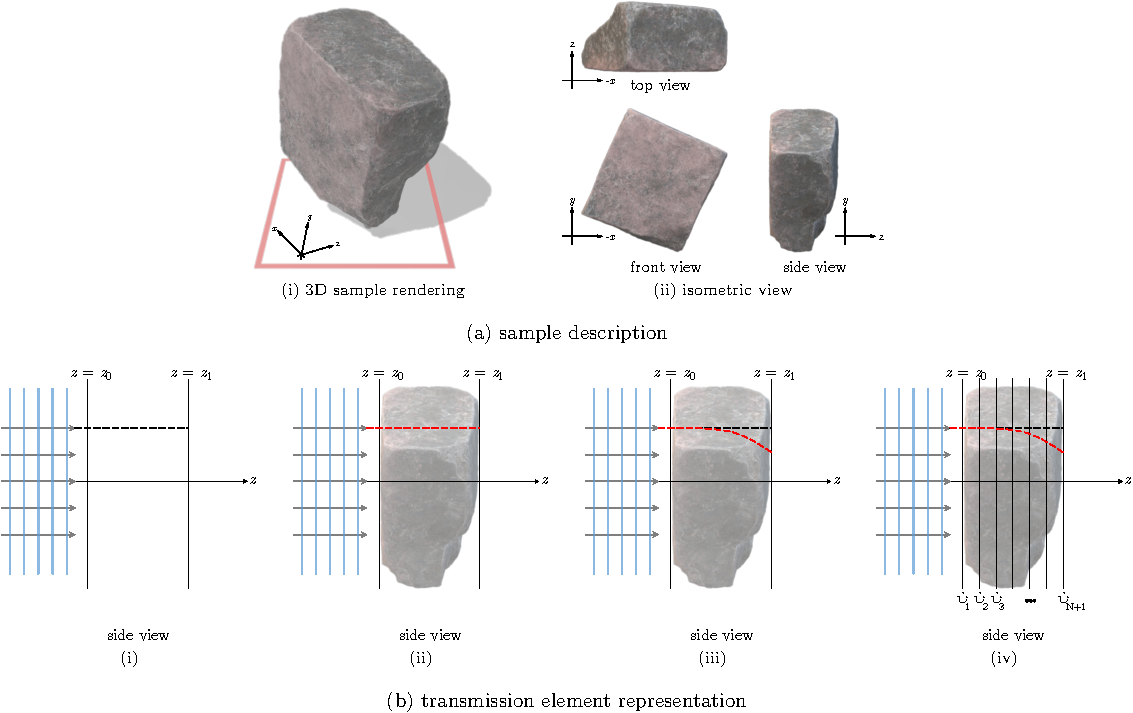
\includegraphics[width=0.9\linewidth]{figures/ch02/projection_approx.pdf}}
    \caption[Transmission elements]{(a) arbitrary-shaped scattering volume in free-space. (b) transmission element representation of said scatterer. The 3D model was taken from the \textit{3D shapes} library in the Paint 3D software from the Microsoft Corporation.}
    \label{fig:projection}
\end{figure}
Consider an arbitrary-shaped scattering volume as shown in Fig.~\ref{fig:projection}(a). Suppose that such scatterer is completely confined within a region $z_0\leq z\leq z_1$ and outside that there is vacuum. Let this sample be illuminated by a plane-wave moving along the positive direction of the optical axis ($z-$axis). In the absence of the scatterer, the gradient between the $z=z_0$ and $z=z_1$ planes is very well defined and parallel to the optical axis, as shown in Fig.~\ref{fig:projection}(b-$\mathrm{i}$). It follows from [\cite[\textit{§2.2}]{Paganin2006}] that if the scatterer is sufficiently weak as to minimally disturb the path that the wave-field would have taken in its absence, cf. Fig.~\ref{fig:projection}(b-$\mathrm{ii}$), the transmission of a wave-field through this sample is given by:
\begin{equation}\label{eq:transmission_n}
    U(x,y,z_1)\approx\exp\Bigg\{-\frac{ik}{2}\int\limits_{z=z_0}^{z=z_1}{\big[1-n^2(x,y,z)\big]~\mathrm{d}z}\Bigg\}U(x,y,z_0).
\end{equation}{}
Eq.~\ref{eq:transmission_n} shows that the effect of a weak scatterer can be accounted by a multiplicative complex transmission element represented by the complex exponential. In the X-ray regime the index of refraction is typically very close to the unity and often expressed as $n=1-\delta+i\cdot\beta$ [\cite[\textit{§1.6}]{Als-Nielsen2011}], which allows for the approximation $1-n(x,y,z)^2\approx2\big[\delta(x,y,z)+i\cdot\beta(x,y,z)\big]$ that can be substituted in Eq.~\ref{eq:transmission_n}. The $z-$dependence of $\delta$ and $\beta$ is abandoned in the projection approximation, hence the complex transmission element in Eq.~\ref{eq:transmission_n} can be reduced to:
\begin{align}\label{eq:transmission}
\mathrm{T}(x,y,z) &=\exp\Bigg\{-ik\int\limits_{z=z_0}^{z=z_1}{\big[\delta(x,y)+i\cdot\beta(x,y)\big]~\mathrm{d}z}\Bigg\}\nonumber\\
         &=\exp\Bigg\{-ik\big[\delta(x,y)+i\cdot\beta(x,y)\big]\Delta_z(x,y)\Bigg\},\nonumber\\
\mathrm{T}\big[\Delta_z(x,y)] &=\sqrt{\mathrm{T}_\text{BL}(x,y)}\exp{\big[i\phi(x,y)\big]}.
\end{align}{}
and:
\begin{subequations}
\begin{align}   
    \mathrm{T}_{\text{BL}}(x,y)&=\exp{\big[-2k\beta(x,y)\Delta_z(x,y)\big]}\label{eq:aux_funcs_transa}  \\
    &=\exp{\big[-\mu(x,y)\Delta_z(x,y)\big]},\nonumber\\
    \phi(x,y)&=-k\delta(x,y)\Delta_z(x,y).\label{eq:aux_funcs_transb}
\end{align}
\end{subequations}
$\Delta_z$ is the projected thickness along the $z-$axis and it depends on the transverse coordinates $(x,y)$, which can be dropped out for a more concise representation. Because of the multiplicative nature of the transmission element, Eq.~\ref{eq:transmission} can be put in operator\footnote{Using the operator formulation was inspired by discussions with David Paganin (Monash University, Australia) and Vincent Favre-Nicolin (ESRF, France).} form:
\begin{equation}\label{eq:transmission_operator}
    \mathrm{T}(\Delta_z)~\bullet =\sqrt{\mathrm{T}_\text{BL}(\Delta_z)}\exp{(-i\phi\Delta_z)}~\bullet.
\end{equation}
Eq.~\ref{eq:aux_funcs_transa} shows the absorption experienced by the wave-field when passing through matter (Beer-Lambert law) and Eq.~\ref{eq:aux_funcs_transb} shows the phase-shift experienced by the wave-field. The coefficient multiplying $\Delta_z$ in $\mathrm{T}_{\text{BL}}$ is know as linear attenuation coefficient $\mu$ [\cite[\textit{§1.6}]{Als-Nielsen2011}]. 

%-------------------------------------------------------------------------
%-------------------------------------------------------------------------
\subsubsection*{The multi-slice approximation}
%-------------------------------------------------------------------------
%-------------------------------------------------------------------------

For the cases where the projection approximation may not be adequate to correctly represent the scattering volume in question, multi-slicing techniques (MS) can be used for describing the wave-field propagation inside an arbitrary-shaped scattering volume - cf. discussion in [\cite[\textit{§2.7}]{Paganin2006}], [\cite{Li2017}] and [\cite{Munro2019}].

Consider the scatterer depicted in Fig.~\ref{fig:projection}(a). If its presence considerably disturbs the path that the wave-field would have taken in its absence, cf. Fig.~\ref{fig:projection}(b-$\mathrm{iii}$), it is possible to section the sample into a number $N$ of parallel slabs until the projection approximation is valid between two adjacent slices - Fig.~\ref{fig:projection}(b-$\mathrm{iv}$). The projected thickness $\Delta_z$ to be used in Eq.~\ref{eq:transmission} is the one in the between slices, which are $\Delta_S=(z_1 - z_0)/N$ apart from each other. Each slice represented as a thin element in projection approximation is separated by vacuum. The propagation of a wave-field propagation through this sample is done step-wise, where each step is composed of a multiplication by a complex transmission element in projection approximation (cf. Eq.~\ref{eq:transmission}) and a Fresnel free-space propagation (Eq.~\ref{eq:Fresnel}) over a distance $\Delta_S$. The output field from this operation is again multiplied by complex transmission element in projection approximation followed by a free-space propagation from the plane $\psi_j$ to the  $\psi_{j+1}$ - refer to Fig.~\ref{fig:projection}(b-$\mathrm{iv}$). This operation is done recursively $N$ times until the wave-field emerges from the sample. The multi-slicing transmission operator can be written in operator form as:
\begin{align}\label{eq:MS}
    \mathrm{T}_\text{MS}=\prod\limits_{j=1}^{N}\mathcal{D}(\Delta_S)\big[\mathrm{T}_j(\Delta_z)~\bullet\big]
\end{align}{}
where $\prod$ indicates concatenation of operators to be performed from right to left, $\mathcal{D}(\Delta_S)$ is the operator formulation of the Fresnel free-space propagation over a distance $\Delta_S$:
\begin{equation}\label{eq:Fresnel_operator}
    \mathcal{D}(\Delta_S)~\bullet=\frac{k\exp{(ik\Delta_S)}}{2\pi i \Delta_S}\iint\limits_{-\infty}^{\hspace{8pt}\infty}{\bullet~\exp{\Bigg\{\frac{ik}{2\Delta_S}\big[(x_1-x)^2+(y_1-y)^2 \big]\Bigg\}}~\mathrm{d}x\mathrm{d}y},
\end{equation}
and $\mathrm{T}_j(\Delta_z)$ is the $j-$th complex transmission element operator in projection approximation associated with the $j-$th slice given by Eq.~\ref{eq:transmission_operator}.

%-------------------------------------------------------------------------
%-------------------------------------------------------------------------
\subsubsection*{-- On the validity of the Fresnel approximation for short propagation distances\footnote{The author acknowledges the fruitful discussions with David Paganin (Monash University, Australia), Peter Munro (University College London, England) and Oleg Chubar (Brookhaven National Lab., USA) when investigating the application of the Fresnel approximation for short propagation distances.}}
%-------------------------------------------------------------------------
%-------------------------------------------------------------------------

A case of particular importance for X-ray optical design is the is application of the Fresnel propagators in real or reciprocal space to very short propagation distances (from millimetres to hundreds of micrometres) at hard X-ray energies (wavelength of the order of the \r{A}ngstrom) with physical apertures of the order of the millimetre. For situations of practical interest such as the one just described, Eq.~\ref{eq:accuracy_Fresnel} is generally very restrictive. This section presents conditions under which said constraint can be relaxed and even overlooked. 

Consider an X-ray wavefield with wavelength $\lambda=1~\AA$ fully illuminating an aperture $A=500~\mu$m situated at $z=z_0$ along the optical axis as shown in Fig.~\ref{fig:diffraction}. The X-rays passing through such an aperture will illuminate an identical aperture $A$ at a distance $z_1-z_0=L$. Suppose one wants to place the second aperture a distance $L$ such as it is possible to calculate the field distribution in $z_1$ using the Fresnel diffraction integral in Eq.~\ref{eq:Fresnel}. Using Eq.~\ref{eq:accuracy_Fresnel} with the extreme points\footnote{For simplicity, the 1D case is analysed, but the conclusions are easily translated to a 2D system if $U(x,y)=U(x)U(y)$.} given by $(x_0=-A/2, y_0=0)$ and $(x_1=A/2, y_1=0)$, one concludes that $ L\gg86~$mm. However, if one wants to place the second aperture at a distance of $L=1$~mm and still be able to safely apply Eq.~\ref{eq:Fresnel} to calculate the field distribution in $z_0$, the apertures should be reduced to $A\ll18~\mu$m according to Eq.~\ref{eq:accuracy_Fresnel}. The situation just described is at odds with the employment of the Fresnel propagator for very short propagation distances at hard X-ray energies with physical apertures of the order of the millimetre. Yet, with the exception of [\cite{Ali2020}], that explicitly uses the Huygens-Fresnel principle [\cite[\textit{\S3.7}]{Goodman2017}] in its reciprocal form for the wavefield propagation\footnote{cf. Eq.~22 or procedure \textit{PropShort} in Algorithm 1 from [\cite{Ali2020}].}, authors make extensive use of the Fresnel propagator for multi-slicing applications under said conflicting conditions [\cite{Li2017, Munro2019, Celestre2020}]. Possibly one of the few explicit mentions of the propagation distance relation to the transverse plane size applied to multi-slicing techniques is given by Eq.~15 in [\cite{Ishizuka1977}]. It turns out that, indeed, Eq.~\ref{eq:accuracy_Fresnel} when applied to a collimated beam (either a plane-wave or a slowly diverging/converging wave) is too restrictive and can be overlook when applied to MS modelling of weak scatteres.

In an early study where the Fresnel diffraction integral (Eq.~\ref{eq:Fresnel}) is directly compared with the Huygens-Fresnel integral (Eq.~\ref{eq:Huygens-Fresnel}) in terms of amplitude and phase, it was shown that the Fresnel approximation has good accuracy: within 2\% in amplitude and 0.02~rad in phase, when compared to the Huygens-Fresnel integral [\cite{Southwell1981}]. The findings hold even for very high Fresnel numbers\footnote{The Fresnel number is defined as $N_F=a^2/\lambda L$, where $a$ is the half aperture, $\lambda$ is the wavelength and $L$ is the propagation distance. A high Fresnel number indicates the region know as near-field, while the far-field region is know for its low Fresnel numbers. In [\cite{Southwell1981}], it is reported that even for $L<a$ good agreement between the Fresnel approximation and the Huygens-Fresnel integral is found for a point within the projected aperture.} along the optical axis within the projected aperture, that is, $\forall~(x,y) \in A$ - [cf. Figs.~1--4 ibid.]. However, for points outside that region ($\forall~(x,y) \notin A$) at very high Fresnel numbers (shadow region), the approximation breaks down: although the amplitude calculation retains good agreement, the phase errors become unacceptably high [cf. Fig.~10 ibid.]. 

\begin{figure}[t]
    \centering
    {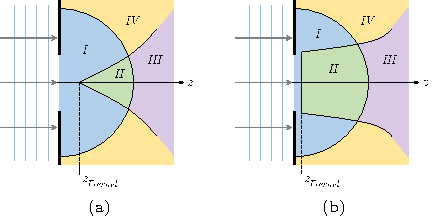
\includegraphics[width=0.6\linewidth]{figures/ch02/Fresnel.pdf}}
    \caption[The validity of the Fresnel approximation]{The Fresnel and Fraunhofer approximations region of validity according to the (a) Eqs.~\ref{eq:accuracy_Fresnel} and \ref{eq:accuracy_Fraunhofer}. For a gently divergent, convergent or plane wavefield the constraints can be relaxed, increasing the region o applicability of said approximations. Region \textit{I} represents the shadow zone, where neither approximations are valid. Region \textit{II} is where only the Fresnel approximation is valid. In region \textit{III}, both approximations coexist, the Fraunhofer being advantageous computationally. Region \textit{IV} illustrates an area where only the Fraunhofer approximation is valid - this counter-intuitive result is discussed in [\cite{Rees87}], but is out of the scope here. The boundaries between regions \textit{I} and \textit{II} have been exaggerated for clarity. This figure is adapted from Fig.~4 and Fig.~5 in [\cite{Rees87}].}
    \label{fig:validity_fresnel}
\end{figure}

Another study that confirms the validity of the Fresnel approximation for a collimated beam being propagated over a very short distance in presented by [\cite{Rees87}]. This work not only confirms the numerical findings in [\cite{Southwell1981}], but also provides physical explanations, some analytical formulations and derives quantitatively the shape of the region where the Fresnel approximation is valid. By applying directly Eq.~\ref{eq:accuracy_Fresnel} and  Eq.~\ref{eq:accuracy_Fraunhofer}, one obtains the the regions of validity for both Fresnel and Fraunhofer integrals as in Fig.~\ref{fig:validity_fresnel}(a), in which case, $z_{Fresnel}$ is given by Eq.~\ref{eq:accuracy_Fresnel} - cf. Eq.~7 in [\cite{Rees87}]. The relaxing of such constrains is done by invoking the concept of Fresnel zones\footnote{cf. [\cite{Hetch}]} and how much contribution it has to the total amplitude and phase of the propagated beam. Considering that the first zone is unobstructed by the aperture $A$, which is the case for all points not within the shadow region, the distance where the Fresnel diffraction integral starts to be accurate can be as low as $z_{Fresnel}=2\lambda$ - cf. Eq.~9 in [\cite{Rees87}]. This is relaxed regime is represented in Fig.~\ref{fig:validity_fresnel}(b).

Based on the results from [\cite{Southwell1981}] and [\cite{Rees87}], it is possible to affirm that provided the object is illuminated with a plane wave and the output field is calculated in the vicinity of the projected aperture, the application of the Fresnel diffraction integral to very short propagation distances for hard X-ray optics modelling with MS techniques is not limited to the constraints imposed by Eq.~\ref{eq:accuracy_Fresnel}. Cases of interest often have non-plane-wave illumination and require special handling to ensure MS with the Fresnel diffraction integral yields accurate results. Approaches that rely on spherical-to-plane-wave conversion are often employed to avoid such accuracy issues: the angular spectrum of plane waves decomposition [\cite[\textit{\S1.3}]{Paganin2006}]\footnote{Also in [\cite[\textit{\S3.10}~\&~\textit{\S4.2.4}]{Goodman2017}].}, the Fresnel-scaling theorem [\cite[\textit{\S A}]{Paganin2006}], the divergent-beam-to-plane-wave transformation from [\cite{Munro2019}] and the analytical treatment of the quadratic phase term [\cite{Chubar2019}], which is of particular interest within the context of this work, as it is the chosen method for the free-space wavefront propagation simulations presented here. 

%-------------------------------------------------------------------------
%-------------------------------------------------------------------------
\subsubsection*{\normalsize -- Real and reciprocal space Fresnel propagators at short propagation distances }
%-------------------------------------------------------------------------
%-------------------------------------------------------------------------

Because of the equivalency of the Fresnel diffraction integral (Eq.~\ref{eq:Fresnel}) and the convolution integral (Eq.~\ref{eq:conv}), one can define the kernel of the Fresnel transform in real-space as:
\begin{align}\label{eq:kernel_real}
    h(x,y)=\exp\bigg[\frac{i\pi}{\lambda L}\big(x^2+y^2 \big)\bigg],
\end{align}{}
while the kernel of the Fresnel transform in reciprocal-space is given by:
\begin{align}\label{eq:kernel_reciprocal}
    H(f_x,f_y)=\exp{\bigg[-i\pi\lambda L\big(f_x^2+f_y^2 \big)\bigg]}.
\end{align}{}
The Eqs.~\ref{eq:kernel_real} and \ref{eq:kernel_reciprocal} are related by: $H(f_x,f_y)=i/(\lambda L) \mathcal\cdot{F}\{ h(x,y)\}$ (cf. Eq.~\ref{eq:kernel}). When propagating a wave-field over a very small distance $L$ with the Fresnel diffraction integral, the argument of the exponential function in transformation kernel in real-space becomes very large and the kernel becomes less well-behaved as shown in  Fig.~\ref{fig:real_reciprocal}(a)-(b), consequently small propagation distances are better represented in the reciprocal space - cf. Fig.~\ref{fig:real_reciprocal}(c)-(d). This hints to the fact that when numerically evaluating the Fresnel transform for short propagation distances, methods using the reciprocal-space are more advantageous than in real-space and constrains like the Eq.~\ref{eq:accuracy_Fresnel} can be overlooked provided the non-paraxial components of the Fourier spectrum of the input wavefield is negligible.

\begin{figure}[t]
    \centering
    {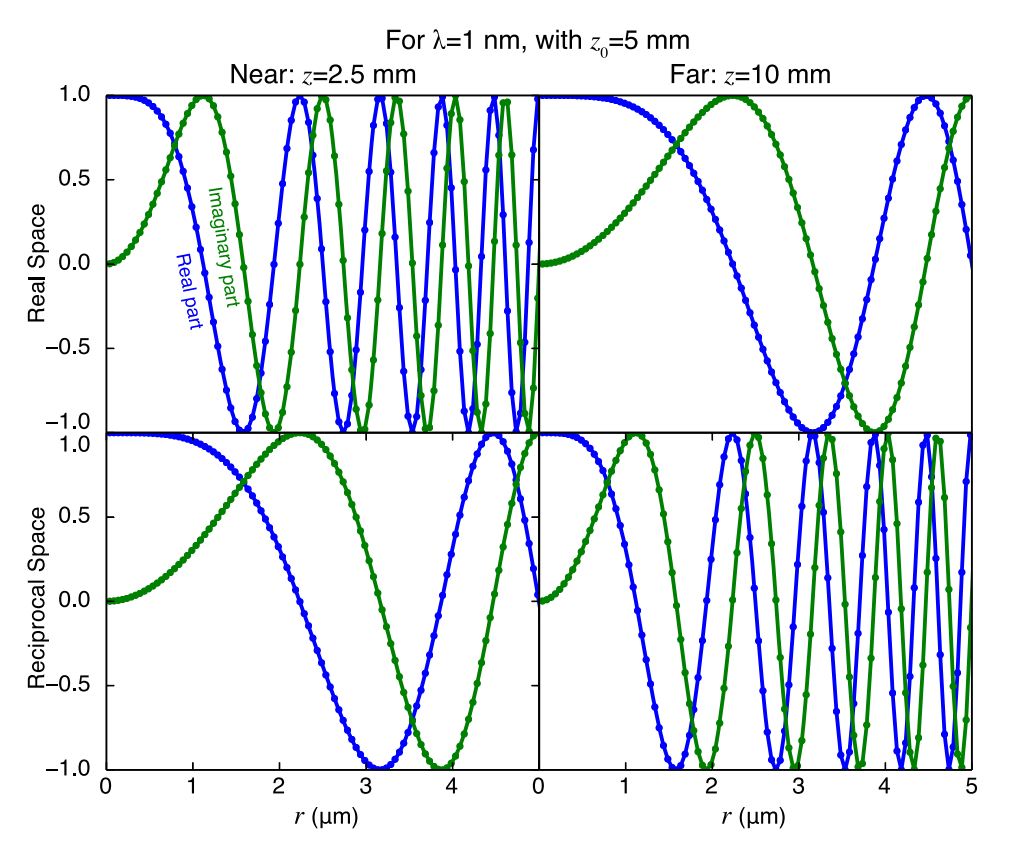
\includegraphics[width=0.6\linewidth]{figures/ch02/real_reciprocal.png}}
    \caption[Frensel transformation kernel in real and reciprocal space]{Real-space kernel of the Fresnel transformation for (a) a short propagation distance and for a (b) longer propagation distance. The reciprocal-space propagator kernel is shown in (c) for a small propagation distance and in (d) for a longer distance. Adapted from Fig.~1 in [\cite{Li2015}].}
    \label{fig:real_reciprocal}
\end{figure}
%-------------------------------------------------------------------------
%-------------------------------------------------------------------------
\subsubsection*{\normalsize -- The analytical treatment of the of the quadratic radiation phase term\footnote{The analytical treatment of the of the quadratic radiation phase terms was introduced in 2007 for the SRW code [\cite{Chubar2008}] (cf. §\ref{sec:wave_propag} in §\ref{sec:optical_simulations}~-~\textit{\nameref{sec:optical_simulations}}). A more detailed description of the memory and CPU efficient computation of the Fresnel free-space propagator in Fourier optics simulations is given by [\cite{Chubar2019}], from which this section is partially based on.}}
%-------------------------------------------------------------------------
%-------------------------------------------------------------------------

Consider a non-collimated wave-field $U(x_0,y_0,z_0)$ in free-space (eg. Eq.~\ref{eq:spherical} or Eq.~\ref{eq:gaussian}). The phase term of such wave has quadratic terms with radii of curvature in the horizontal and vertical planes $R_x$ and $R_y$ and the transverse coordinates of the centre point $(x_\text{c},y_\text{c})$. It is possible to rewrite $U(x_0,y_0,z_0)$ as:
\begin{align}\label{eq:Semi_a}
    U(x_0,y_0,z_0) = F(x_0,y_0,z_0)\exp{\Bigg\{\frac{ik}{2}\Bigg[\frac{(x_0-x_c)^2}{R_y}+\frac{(y_0-y_c)^2}{R_y} \Bigg]\Bigg\}},
\end{align}{}
where $F(x_0,y_0,z_0)$ is the residual wavefront after the quadratic phase term is factorised. This residual wave-field satisfies the necessary conditions for the compliance with the Fresnel propagation of collimated beams through very short propagation distances as required by [\cite{Southwell1981}] and [\cite{Rees87}]. Substituting Eq.~\ref{eq:Semi_a} in the Fresnel diffraction integral (Eq.~\ref{eq:Fresnel}):
\begin{multline}\label{eq:Semi_b}
    U(x_1,y_1,z_1)=\frac{k\exp{(ikL)}}{2\pi i L}\iint\limits_{-\infty}^{\hspace{8pt}\infty}{F(x_0,y_0,z_0)}\cdot\\ \cdot{\exp{\Bigg\{\frac{ik}{2}\Bigg[\frac{(x_1-x_0)^2+(y_1-y_0)^2}{L}+\frac{(x_0-x_c)^2}{R_y}+\frac{(y_0-y_c)^2}{R_y} \Bigg]\Bigg\}}~\mathrm{d}x_0\mathrm{d}y_0},
\end{multline}
which can be conveniently expressed as: 
\begin{align}\label{eq:Semi_c1}
    U(x_1,y_1,z_1) = F(x_1,y_1,z_1)\exp{\Bigg\{\frac{ik}{2}\Bigg[\frac{(x_1-x_c)^2}{R_y+L}+\frac{(y_1-y_c)^2}{R_y+L} \Bigg]\Bigg\}},
\end{align}{}
with:
\begin{multline}\label{eq:Semi_c2}
    F(x_1,y_1,z_1)=\frac{k\exp{(ikL)}}{2\pi i L}\iint\limits_{-\infty}^{\hspace{8pt}\infty}{F(x_0,y_0,z_0)}\cdot\\ \cdot{\exp{\Bigg\{\frac{ik}{2L}\Bigg[\frac{R_x + L}{R_x}\Bigg(\frac{R_xx_1+Lx_c}{R_x+L} - x_0\Bigg)^2+\frac{R_y + L}{R_y}\Bigg(\frac{R_yy_1+Ly_c}{R_y+L} - y_0\Bigg)^2\Bigg]\Bigg\}}~\mathrm{d}x_0\mathrm{d}y_0}.
\end{multline}
It is evident that much like Eq.~\ref{eq:Fresnel}, Eq.~\ref{eq:Semi_c2} is a convolution-type integral with analytical Fourier transform of the convolution kernel, hence the discussion presented in \textit{Numerical computation of the Fresnel and Fraunhofer diffraction} in \S\ref{sec:free-space}~-~\textit{\nameref{sec:free-space}} is still applicable and the advantages of the wave propagation at very short distances in reciprocal space are maintained. The analytical treatment of the of the quadratic radiation phase term reduces significantly the required transverse sampling of the wave-field without compromising the compromising the accuracy of calculation, as the oscillations of the residual electric field are less rapid and require less dense sampling. Another advantage of such rewriting of the Fresnel diffraction integral is that the convolution shown in Eq.~\ref{eq:Semi_c2} takes place with respect to the scaled transverse coordinates $x_1\cdot R_x/(R_x+L)$ and $y_1\cdot R_y/(R_y+L)$. When using the convolution-theorem formulation of free-space propagation (cf. Eqs.~\ref{eq:conv} and \ref{eq:conv_theorem}), the scaled coordinates re-scale without any additional re-sampling nor interpolation the output plane by $\Delta x_1 = \Delta x_0 \cdot (R_x+L)/R_x$ and  $\Delta y_1 = \Delta y_0 \cdot (R_y+L)/R_y$, where $\Delta x_0$ and $\Delta y_0$ are the input plane dimensions. The formulation shown in Eqs.~\ref{eq:Semi_c1} and \ref{eq:Semi_c2} has singularities at $R_x+L = 0$ and $R_y+L = 0$, which happens when calculating the propagation of a wavefront after a focusing element at the image plane. The singularities can be dealt with by simply applying a $R_x'\neq0$ and $R_y'\neq0$ such as they are near $R_x$ and $R_y$, but avoid the singularity. Using  $R_x'\neq0$ and $R_y'\neq0$ still reduces the required transverse sampling and re-scales the output plane when propagating the wave-field by using the convolution-theorem formulation.

%-------------------------------------------------------------------------
%-------------------------------------------------------------------------
\subsection{Optical coherence}\label{sec:optical_coherence}
%-------------------------------------------------------------------------
%-------------------------------------------------------------------------

Within the context of accelerator-based X-ray sources, more specifically, undulators in storage rings, it has been shown previously that increasing the brilliance of the X-rays by emittance matching (cf. Eq.~\ref{eq:emittances} and Fig.\ref{fig:matching}) implies increasing the coherent fraction of the emitted X-rays (Eq.~\ref{eq:coherent_fraction}). Later on, this increased coherent flux was used to justify using physical optics among the optical theories (Fig.~\ref{fig:optical_theories}) to provide a framework for describing X-rays propagation in free-space and within matter. The word coherence, be it temporal or spatial, has been used throughout this work but without a clear definition. This section should clarify its concept in the context of synchrotron radiation and provide some basic definitions\footnote{The developments shown in this section are based on [\cite[\textit{§4}]{Mandel1995}].}.

%-------------------------------------------------------------------------
%-------------------------------------------------------------------------
\subsubsection*{Mutual coherence function}
%-------------------------------------------------------------------------
%-------------------------------------------------------------------------

Emission of synchrotron radiation is a fundamentally random process and as such, it should be treated probabilistically. It has been demonstrated by [\cite{Geloni2008}] that although SR is intrinsically not stationary\footnote{A statistical process is stationarity if all ensemble averages are independent of time, which is not the case for synchrotron radiation. The averaging brackets $\langle \bullet \rangle$ indicate average over the bunches instead.} nor homogeneous\footnote{Homogeneity implies a constant ensemble-averaged intensity along the transverse direction.}, under realistic conditions (practical cases of interest) SR can be considered quasi-stationary and quasi-homogeneous thus the formalism of statistical optics can be applied.

Consider an arbitrary complex scalar wave-field $u(\textbf{r},t)$, where $\textbf{r}=(x,y,z)$, satisfying the wave-equation \ref{eq:Scalar_WE}. The correlation between the spatial and temporal fluctuations of $u(\textbf{r},t)$ at two different positions in space, that is $\textbf{r}_1 = (x_1,y_1,z_1)$ and $\textbf{r}_2 = (x_2,y_2,z_2)$, and separated by a time delay $\tau=t_2-t_1$ is given by the mutual coherence function\footnote{cf. Eq.~4.3-6 in [\cite{Mandel1995}].} (MCF):
\begin{equation}\label{eq:MCF}
    \Gamma(\textbf{r}_1,\textbf{r}_2,\tau) = \big\langle u^*(\textbf{r}_1,t)u(\textbf{r}_2,t+\tau)\big\rangle,
\end{equation}
where $\bullet^*$ indicates the complex conjugate. The normalised form of this cross-correlation function (Eq.~\ref{eq:MCF}) is called the complex degree of coherence\footnote{cf. Eq.~4.3-12a in [\cite{Mandel1995}].} (CDC):
\begin{equation}\label{eq:CDC}
    \gamma(\textbf{r}_1,\textbf{r}_2,\tau) = \frac{\Gamma(\textbf{r}_1,\textbf{r}_2,\tau)}{\sqrt{\Gamma(\textbf{r}_1,\textbf{r}_1,0)\Gamma(\textbf{r}_2,\textbf{r}_2,0)}},
\end{equation}
where the averaged intensity at a point $\textbf{r}$ is given by: $\big\langle I(\textbf{r},t)\big\rangle = \big\langle u^*(\textbf{r},t)u(\textbf{r},t)\big\rangle = \Gamma(\textbf{r},\textbf{r},0)$. The absolute value of Eq.~\ref{eq:CDC} is limited: $0\leq|\gamma(\textbf{r}_1,\textbf{r}_2,\tau)|\leq 1$, where $|\gamma|=0$ means total uncorrelation and $|\gamma|=1$ denotes full correlation of the fluctuations at positions  $\textbf{r}_1 = (x_1,y_1,z_1)$ and $\textbf{r}_2 = (x_2,y_2,z_2)$ temporally separated by $\tau$ [\cite[\textit{§11}]{Saleh2019}]. The extreme cases of $|\gamma(\textbf{r}_1,\textbf{r}_2,\tau)|=0$ and $|\gamma(\textbf{r}_1,\textbf{r}_2,\tau)|=1$ are known as fully-incoherent and fully-coherent cases and all values in between those imply partially coherent radiation. Eq.~\ref{eq:CDC} is connected to the cross-spectral density (CSD) by a Fourier transform\footnote{Wiener–Khinchin theorem - cf. §2.4 in [\cite{Mandel1995}].} with respect to $\tau$:
\begin{equation}\label{eq:CSD}
    W(\textbf{r}_1,\textbf{r}_2,\omega)=\int\limits_{-\infty}^\infty{\Gamma(\textbf{r}_1,\textbf{r}_2, \tau)\exp{(-i\omega t)}~\mathrm{d}\tau}.
\end{equation}{}
The normalised cross-spectral density function\footnote{cf. Eq.~4.3-47a in [\cite{Mandel1995}].} is given by:
\begin{equation}\label{eq:SDC}
    \mu(\textbf{r}_1,\textbf{r}_2,\omega)=\frac{W(\textbf{r}_1,\textbf{r}_2,\omega)}{\sqrt{W(\textbf{r}_1,\textbf{r}_1,\omega)W(\textbf{r}_2,\textbf{r}_2,\omega)}}.
\end{equation}{}
Eq.~\ref{eq:SDC} is known as the spectral degree of coherence (SDC) and much like the absolute value of Eq.~\ref{eq:CDC}, it is bounded by $0\leq|\mu(\textbf{r}_1,\textbf{r}_2,\omega)|\leq 1$. Although the mutual coherence function (Eq.~\ref{eq:MCF}) and the cross-spectral density (Eq.~\ref{eq:CSD}) are connected by a Fourier transform, the complex degree of coherence (Eq.~\ref{eq:CDC}) and the spectral degree of coherence (Eq.~\ref{eq:SDC}) are not [\cite[\textit{§4.3.2}]{Mandel1995}].

A well known result from coherence theory and the cross-spectral density representation of the mutual coherence function is the coherent mode representation of partially coherent fields in free-space [\cite[\textit{§4.7.1}]{Mandel1995}]. It is possible to decompose the CSD in a infinite sum of coherent modes\footnote{cf. Eq.~4.7-9 in [\cite{Mandel1995}].}:
\begin{equation}\label{eq:CMD}
    W(\textbf{r}_1,\textbf{r}_2,\omega)=\sum\limits_{j=1}^\infty{\alpha_j(\omega)\Phi^*_j(\textbf{r}_1,\omega)\Phi_j(\textbf{r}_2,\omega)},
\end{equation}{}
where $\alpha_j(\omega)$ are the weights (eigenvalues) of the corresponding modes (eigenfunctions) $\Phi_j(\textbf{r},\omega)$. The modes described in Eq.~\ref{eq:CMD}  form an orthonormal set and maximise the CSD, that is, $0\leq \alpha_{j+1}(\omega)<\alpha_j(\omega)$, making the truncation optimal. If the wave-field is completely coherent, it can be represented by a single mode [\cite[\textit{§4.7}]{Mandel1995}]. Defining the mode occupancy as:
\begin{equation}\label{eq:mode_ocupation}
    \eta_m=\frac{\alpha_m(\omega)}{\sum\limits_{j=1}^\infty{\alpha_j(\omega)}},
\end{equation}{}
allows to define the coherent fraction as the occupancy of the first mode $\eta_1$ (cf. Eq.~\ref{eq:coherent_fraction}).

%-------------------------------------------------------------------------
%-------------------------------------------------------------------------
\subsubsection*{Spatial coherence}
%-------------------------------------------------------------------------
%-------------------------------------------------------------------------

In the quasi-monochromatic regime\footnote{Conditions for the quasi-monochromatic regime in the context of SR are discussed in [\cite[\textit{§2.3}]{Geloni2008}].} Eqs.~\ref{eq:MCF}~and~\ref{eq:CDC} can be approximated as:
\begin{align}
    \Gamma(\textbf{r}_1,\textbf{r}_2,\tau) &\approx J(\textbf{r}_1,\textbf{r}_2)\exp{\big(i\omega_0 \tau\big)},\label{eq:Gamma_approx}\\
    \gamma(\textbf{r}_1,\textbf{r}_2,\tau) &\approx j(\textbf{r}_1,\textbf{r}_2)\exp{\big(i\omega_0 \tau\big)}.\label{eq:gamma_approx}
\end{align}{}
The aforementioned approximations (Eqs.~\ref{eq:Gamma_approx} and \ref{eq:gamma_approx}) are valid given that $|\tau|\ll 1/\Delta\omega$, where $\Delta \omega$ is the radiation bandwidth and $\omega_0$ is its centre. The quantities $J(\textbf{r}_1,\textbf{r}_2)\equiv\Gamma(\textbf{r}_1,\textbf{r}_2,0)$ and $j(\textbf{r}_1,\textbf{r}_2)\equiv\gamma(\textbf{r}_1,\textbf{r}_2,0)$ are known as the equal-time-correlation functions\footnote{cf. Eqs.~4.3-31--4.3-35 in [\cite{Mandel1995}].}. $J(\textbf{r}_1,\textbf{r}_2)$ is called the mutual optical intensity (MOI) and $j(\textbf{r}_1,\textbf{r}_2)$ is the complex degree of spatial coherence. The transverse coherence length can be arbitrarily defined as a $\Delta_{\textbf{cl}_\perp}=|\textbf{r}_2-\textbf{r}_1|$ to which $j(\textbf{r}_1,\textbf{r}_2)$ falls below a certain threshold. Alternatively, the transverse coherence length can be approximated by the van-Cittert-Zernike theorem\footnote{The applicability of the van-Cittert-Zernike theorem to SR is discussed in [\cite[\textit{§4}]{Geloni2008}].} - cf. [\cite[\textit{§4.4.4}]{Mandel1995}] and [\cite[\textit{§11.3.C}]{Saleh2019}]. The experiment in classical optics mostly associated with the spatial coherence is the Young's double slit experiment [\cite[\textit{§5.2.1}]{Goodman2015}].

%-------------------------------------------------------------------------
%-------------------------------------------------------------------------
\subsubsection*{Temporal coherence}
%-------------------------------------------------------------------------
%-------------------------------------------------------------------------

Alternatively, Eqs.~\ref{eq:MCF}~and~\ref{eq:CDC} can be evaluated at a fixed position $\textbf{r}$, giving rise to to the (temporal) coherence function and the complex degree of (temporal) coherence, respectively: $\Gamma(\textbf{r},\textbf{r},\tau)$ and $\gamma(\textbf{r},\textbf{r},\tau)$:
\begin{align}
    \Gamma(\textbf{r},\textbf{r},\tau)&=\big\langle u^*(\textbf{r},t)u(\textbf{r},t+\tau)\big\rangle,\label{eq:Gamma_t}\\
    \gamma(\textbf{r},\textbf{r},\tau) &= \frac{\Gamma(\textbf{r},\textbf{r},\tau)}{\Gamma(\textbf{r},\textbf{r},0)}.\label{eq:gamma_t}
\end{align}{}
The Fourier transform of Eq.~\ref{eq:Gamma_t} with respect to $\tau$, $\mathcal{F}\big\{\Gamma(\textbf{r},\textbf{r},\tau)\big\}\equiv S(\textbf{r},\omega)$, is called the spectrum density of the wave-field. Similarly, a longitudinal coherence length can be arbitrarily defined as a $\Delta_{\textbf{cl}_\parallel}=c\tau$ to which $\gamma(\textbf{r},\textbf{r},\tau)$ falls below a certain threshold.
The experiment in classical optics mostly associated with the temporal coherence is the Michelson's interferometer experiment [\cite[\textit{§5.1.1}]{Goodman2015}].

\subsection*{Recommended literature}

A comprehensive introduction to the scalar-wave-theory is presented by [\cite[\textit{§1} \& \textit{§2}]{Paganin2006}] and [\cite{Goodman2017}]. For a deeper look into statistical optics and partially-coherent fields, please, refer to [\cite[\textit{§4}]{Mandel1995}], [\cite[\textit{§10}]{born_wolf1999}] or [\cite[\textit{§5}]{Goodman2015}].

%-------------------------------------------------------------------------
%-------------------------------------------------------------------------
\section{X-ray optical simulations}\label{sec:optical_simulations}
%-------------------------------------------------------------------------
%-------------------------------------------------------------------------

There are several software packages for optical design in the X-ray range\footnote{As opposed to the optical systems design for the visible range, X-ray optical systems can often use strongly off-axis configurations with grazing incidence angles for reflective optics, crystals and other niche-specific optical elements. X-ray sources also differ from common visible light sources and often require special models (bending magnets, wigglers, undulators). Consequently, traditional approaches and commercial software for visible light are often ill-suited for X-ray optical simulations.}: \textit{SHADOW} [\cite{Lai1986}], \textit{McXtrace} [\cite{BergbackKnudsen2013}] and \textit{xrt} [\cite{Klementiev2014}] among others for ray-tracing calculations; and  \textit{PHASE} [\cite{Bahrdt1997}, \textit{SRW} [\cite{Chubar1998}, \textit{WISEr} [\cite{Raimondi2010} and \textit{xrt} [\cite{Chernikov2017}] to name a few wave-propagation codes. From those, \textit{SHADOW} (ray-tracing\footnote{Phase ray-tracing - cf. [\cite{Lee2007,SanchezdelRio2011}].}) and \textit{SRW} (wave-propagation) are by far the most widely used and bench-marked [\cite{Rio2013,Chubar2014}]. The choice of technique for optical beamline\footnote{In accelerator-based X-ray physics, the optical system transporting the radiation from the accelerator to the sample is called beamline.} simulation is based on several criteria, but is usually intimately connected to the expected physical effects to observed, the degree of coherence of the X-rays and the required accuracy [\cite{SanchezdelRio2019}].

In general\footnote{For typical electron-bunch lengths larger than $\sim30~\text{ps}$, high energies and normal monochromatisation conditions [\cite{Geloni2008}].} synchrotron radiation has very poor temporal coherence properties, that is, $|\gamma(\textbf{r},\textbf{r},\tau)|\approx0$. It follows that any reference to coherence in this thesis (or lack thereof) implies spatial coherence.

\begin{figure}[t]
    \centering
    {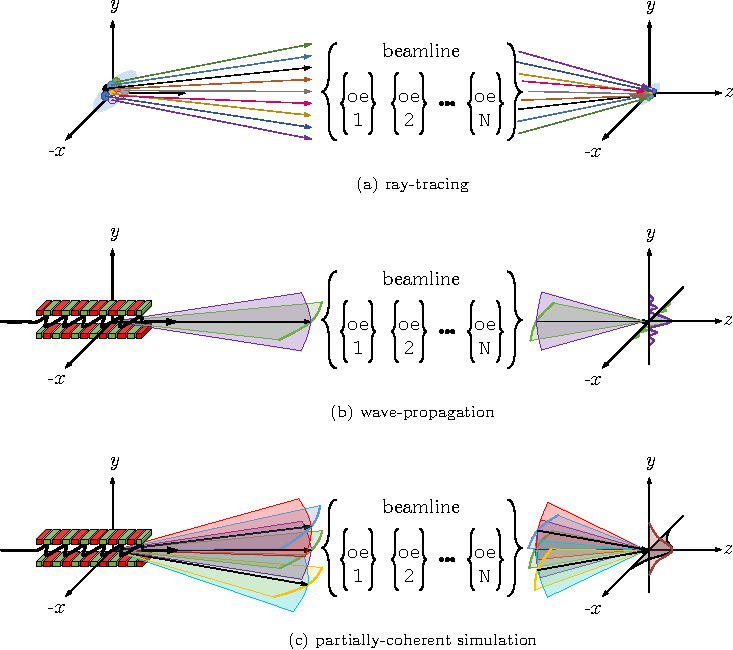
\includegraphics[width=.65\linewidth]{figures/ch02/optical_simulation.pdf}}
    \caption[X-ray optical simulation methods]{X-ray beamline optical simulation methods based on the degree of spatial coherence. A beamline is composed of drift-spaces (free-space) and optical elements (OE). (a) ray tracing methods are more adequate for cases where the degree of spatial coherence is low $\big(|j(\textbf{r}_1,\textbf{r}_2)|\approx0\big)$. (b) When the degree of coherence is close to unity $\big(|j(\textbf{r}_1,\textbf{r}_2)|\approx1\big)$ wave-propagation methods are better suited, as they account for diffraction effects. (c) partially-coherent simulation surpasses the accuracy of pure ray tracing or wave-propagation for cases where $0\ll|j(\textbf{r}_1,\textbf{r}_2)|\ll1$.}
    \label{fig:simulation_methods}
\end{figure}
%-------------------------------------------------------------------------
%-------------------------------------------------------------------------
\subsection{Ray-tracing}\label{sec:ray_tracing}
%-------------------------------------------------------------------------
%-------------------------------------------------------------------------
 For the cases where synchrotron radiation has low spatial coherence, that is, the complex degree of spatial coherence $|j(\textbf{r}_1,\textbf{r}_2)|\approx0$ for a pair of points near opposed edges of the beam footprint, ray-tracing techniques are often employed. The radiation source is simulated by Monte-Carlo sampling of the photon-beam phase-space\footnote{Three spatial coordinates, two transverse angles to describe direction, and the electron-beam energy - the electrons in a storage ring have a Gaussian distribution around a central design energy. The statistical emission of photons is the cause of a change of electron energy leading to energy spread within the electron beam [\cite[\textit{8.3.1}]{Wiedemann2015}].} described by specific numerical models [\cite{Canestrari2013}] and each photon sampled from the source is transported through the beamline using geometrical optics\footnote{Geometric optics is the limit of the physical optics theory when $\lambda$ goes to zero [\cite[\textit{§1.3.C} \& \textit{§2.3}]{Saleh2019}]. In free-space rays propagate in a straight line and have their direction changed by interacting with optical elements. By adding to this pure geometrical model some physical properties, namely, polarisation, intensity and wavelength, it is possible to account for several optical elements based on specular reflection, refraction and diffraction.}. The propagated rays are accumulated at the observation plane. To generate enough statistics and allow the method to converge, several thousands of rays are typically used - cf. Fig.~\ref{fig:simulation_methods}(a). Ray-tracing is a simple and extremely powerful technique for calculating the main characteristics of the photon beam (size, divergence, photon distribution) at every plane along the beamline when diffraction effects are negligible.

%-------------------------------------------------------------------------
%-------------------------------------------------------------------------
\subsection{Wave propagation}\label{sec:wave_propag}
%-------------------------------------------------------------------------
%-------------------------------------------------------------------------

The other extreme is the fully coherent case, that is $|j(\textbf{r}_1,\textbf{r}_2)|\approx1$ for any two pair of points $\textbf{r}_1$ and $\textbf{r}_2$ inside the beam footprint. This regime is often prone to diffraction effects and the framework for dealing with those is best given by wave-propagation, which follows physical optics principles - cf. §\ref{sec:physical_optics}~-~\textit{\nameref{sec:physical_optics}}. The X-ray source can be simply approximated by any solution of the Helmholtz equation (Eq.~\ref{eq:Helmholtz}) or its paraxial form given by Eq.~\ref{eq:Helmholtz_paraxial}. The most commonly used solutions are: the plane wave (Eq.~\ref{eq:planewave}), the spherical wave (Eq.~\ref{eq:spherical}), the parabolic wave (Eq.~\ref{eq:parabolic}) and the Gaussian beam (Eq.~\ref{eq:gaussian}-\ref{eq:gaussian_parameters}). Alternatively, the wavefront emerging from any accelerator-based X-ray source described by an arbitrary magnetic field can be calculated [\cite{Chubar1995, Chubar2001}]. This wave-field can then be propagated in the free-space between the optical elements using the diffraction integrals (cf. Eqs.~\ref{eq:Huygens-Fresnel},  \ref{eq:Fresnel} or \ref{eq:Fraunhofer}). The interaction between the wave and optical elements in the beamline is done by the calculation of the appropriate transmission element\footnote{In addition to the theory describing the propagation of X-rays in the matter (§\ref{sec:thin_element}~-~\textit{\nameref{sec:thin_element}}) a variety of optical elements can be simulated within the wave optics by being able to describe them adequately as transmission elements, similar to a transfer function in signals and systems theory - cf. [\cite{Canestrari2014, Li2017}].}. After the said wave is propagated to the observation plane, the intensity and phase can be calculated. 

%-------------------------------------------------------------------------
%-------------------------------------------------------------------------
\subsection{Partially coherent simulations}\label{sec:partially_coherent}
%-------------------------------------------------------------------------
%-------------------------------------------------------------------------

When doing optical design for X-ray beamlines in synchrotron radiation facilities, there are several cases of interest that are neither well approximated by $|j(\textbf{r}_1,\textbf{r}_2)|\approx0$ nor by $|j(\textbf{r}_1,\textbf{r}_2)|\approx1$ for a pair of points near opposed edges of the beam footprint. Using pure ray-tracing or a single-wave-field propagation to those partially-coherent cases may lead to inaccurate results [\cite{SanchezdelRio2019}]. With varying accuracy, several methods can account for  partially-coherence effects.

%-------------------------------------------------------------------------
%-------------------------------------------------------------------------
\subsubsection*{Hybrid methods}
%-------------------------------------------------------------------------
%-------------------------------------------------------------------------

One class of methods is based on the so-called hybrid methods mixing elements of ray-tracing and wave propagation simulations [\cite{Semichaevsky2001}]. One common approach is to simulate the geometric effects from optical elements with ray-tracing and their diffraction contributions\footnote{Beam clipping by either physical acceptance of an optical element or slits and optical errors.} with wave optics. The diffraction caused by the optical elements is then integrated into ray-tracing by numerical convolution and sampling the calculated wave-front with rays [\cite{Shi2014}]. Another approach is to take into account the optical path followed by individual rays and asserting to them a phase and interpreting them as a localised phase of the wave-front. If sampling is sufficiently high, it is possible to reconstruct a wave-front. These special rays are propagated through the beamline using ray-tracing techniques and are added coherently\footnote{Taking into account their relative phase.} at the observation plane [\cite{Prodi2011}].

%-------------------------------------------------------------------------
%-------------------------------------------------------------------------
\subsubsection*{Physical-optics-based methods}
%-------------------------------------------------------------------------
%-------------------------------------------------------------------------

A second class of methods involves purely wave-front propagation methods. The radiation from the X-ray source can be decomposed in orthogonal modes. These can be propagated though the beamline using the physical optics principles described in §\ref{sec:physical_optics}~-~\textit{\nameref{sec:physical_optics}}. Once the modes are propagated to the observation plane, they can be added in intensity\footnote{cf. Eqs.~\ref{eq:MCF}, \ref{eq:CSD} and \ref{eq:CMD} evaluated for $\textbf{r}=\textbf{r}_1=\textbf{r}_2$ and $\tau=0$.}. X-rays from undulators are commonly decomposed into Gaussian-Schell modes
[\cite{Coisson1997, Singer2011}], which becomes less accurate when dealing with ultra-low emittance machines. More recently, different factorisations have been proposed to accurately represent beams in low-emittance machines [\cite{Lindberg2015, Glass_2017}].

Alternatively, the fact that for high energies the emission from the electrons is uncorrelated can be explored. Each individual electron in a bunch has a different initial condition in terms of position $s=(x_e,y_e,z_e)$, direction $s'=(x'_e,y'_e)$ and energy $\gamma_e$. These electrons spread in the 6D phase-space according to a probabilistic distribution\footnote{The distribution $f(s,s',\gamma_e)$ is intimately connected to the nature of the X-ray source.} $f(s,s',\gamma_e)$ in phase-space such as $\int f(s,s',\gamma_e)~\mathrm{d}x_e\mathrm{d}y_e\mathrm{d}z_e\mathrm{d}x'_e\mathrm{d}y'_e\mathrm{d}\gamma_e=1$. The multi-electron-emission method for partially coherent simulations is based on individually calculating the synchrotron radiation emission of several electrons subjected to the initial conditions sampled from $f(s,s',\gamma_e)$ passing through an arbitrary magnetic field describing the X-ray source [\cite{Chubar1995}]. Each resulting electric field is then propagated through the beamline until the observation point, where the contributions from different electrons are added in intensity. The function $f(s,s',\gamma_e)$ should be statistically well-sampled (Monte-Carlo methods) to guarantee convergence. This multi-electron-emission method was first proposed and implemented by [\cite{Chubar2011}]. This method is shown in Fig.~\ref{fig:simulation_methods}(c).

%-------------------------------------------------------------------------
%-------------------------------------------------------------------------
\subsubsection*{Other methods}
%-------------------------------------------------------------------------
%-------------------------------------------------------------------------

A third class of methods is based on the propagation of the correlation functions\footnote{cf. §\ref{sec:optical_coherence}~-~\textit{\nameref{sec:optical_coherence}}.} through the beamline with methods resembling the ones from physical optics. The theory for such is described in [\cite{Parrent1959}] and [\cite[\textit{§4.4}]{Mandel1995}]. However, these methods are, at the time of this writing, not very commonly applied to X-ray optical simulations due to being very computationally expensive [\cite{Meng2015, Meng2017, Ren2019}] and are certainly not made available on any common software for X-ray optical simulations. $\blacksquare$

\addcontentsline{toc}{section}{References}
\printbibliography[heading=subbibliography]
\end{refsection}

